\chapter{连续函数}
\label{chap:mathematical-analysis}
\label{chap:continuous-functions}

输入逐渐接近一个位置时，函数值能否接近确定的结果？局部的变化率怎样预测有限位移，整个范围内的数值又怎样累计？本章以实数和有限维向量函数为主要对象，研究极限、局部变化与整体累计。第~\ref{chap:sets-functions-and-proofs}章的函数、向量和量词，以及第~\ref{chap:combinatorics}章的增长尺度，是这里表达误差和近似的起点。

这三个问题所需的条件不同。距离和完备性用于判断逼近是否有终点，连续性用于控制输入变化后的输出；微分进一步给出局部线性或高阶近似，积分则累计一个范围内的贡献。我们先分别建立这些工具，再让函数本身组成序列，检查连续性、积分和求导能否传到极限。连续函数是主要入口，不连续或不可微的函数用来说明适用边界。章末的两个问题将留给第~\ref{chap:measurable-functions}章：怎样扩大可积分的函数范围，以及怎样在没有一致误差控制时判断积分极限。

\section{函数的极限与连续性}
\label{sec:analysis-continuous-limits}

本节研究对象怎样接近极限，以及输入趋近时输出怎样变化。逐项能够计算不保证序列有极限，每点连续也不保证整个范围具有共同的误差阈值。下面先用距离和序列区分极限的含义与存在条件，再把这种接近用于函数，最后研究定义域怎样保证极值达到与一致控制。

\subsection{序列的接近与极限存在}
\label{sec:analysis-sequences-series-errors}

数列$1/n$接近$0$，$(-1)^n$却始终振荡。要把这一区别推广到向量和其他对象，我们先规定比较距离，再说明怎样趋向一个候选极限。柯西条件进一步只比较序列尾部，使不知道终点时也能判断是否具备收敛的基础；闭性则检查所得终点是否仍在允许范围内。

\subsubsection{对象之间的接近程度}

\paragraph{实数与向量的距离}

实数之差的绝对值给出一种距离：在实数轴上，两个数之差的绝对值越小，它们越接近。
这一度量只适用于实数；机器学习里还要比较两个特征向量、两条预测曲线甚至两个概率分布是否
接近。为了让“接近”在这些不同对象上都有统一含义，我们把绝对值距离所满足的直观性质
抽出来，要求任何“距离”都遵守它们。可以要求距离满足三条共同规则：零距离能够辨认同一对象，交换对象不改变距离，经过第三个对象的距离之和不小于直接距离。满足这些规则的函数称为度量。
\begin{definition}[度量与度量空间]
\label{def:analysis-metric-space}
集合$X$上的\term{度量}（metric）是函数$d:X\times X\to[0,\infty)$，满足对任意$x,y,z\in X$，
\[
  \begin{aligned}
    d(x,y)=0&\Longleftrightarrow x=y,\\
    d(x,y)&=d(y,x),\\
    d(x,z)&\leq d(x,y)+d(y,z).
  \end{aligned}
\]
带有度量的集合$(X,d)$称为\term{度量空间}（metric space）。
\end{definition}
三条规则各管一件事。第一条要求距离能把不同对象区分开：只有同一个点距离才为零，否则两个不同的点在任何比较中都无法区分。第二条保证“接近”是对称的。第三条不要求距离沿直线累加，只要求绕路不比直达更近，由此得到分析中常用的一条推理：把误差分成几段分别控制，总误差不超过各段之和。式中的范数$\lVert\cdot\rVert_2$在第~\ref{chap:sets-functions-and-proofs}章已定义为向量各坐标平方和的平方根，$\lVert\bm{x}-\bm{y}\rVert_2$就是两个向量对应坐标之差的平方和再开方。

欧氏空间使用$d(\bm{x},\bm{y})=\lVert\bm{x}-\bm{y}\rVert_2$；有限集合可以使用离散度量$d(x,y)=\mathbb{I}\{x\neq y\}$。这里使用的度量都取有限的非负实数，因此$d$的值域写成$[0,\infty)$。同一个集合选择不同度量，可能改变何谓收敛以及函数是否连续；不过，有些度量只改变数值尺度，例如$d$与$2d$具有相同的收敛序列和连续映射。不能仅凭距离公式不同就断言这些性质不同。

\begin{definition}[开球]
\label{def:analysis-open-ball}
在度量空间$(X,d)$中，以$x\in X$为中心、半径$r>0$的开球记为
$B(x,r)=\{y\in X:d(x,y)<r\}$。
\end{definition}

开球把“离一个点足够近”写成集合。若$V\subseteq X$包含某个$B(x,r)$，就称
$V$是$x$的邻域；邻域本身不必是开集。由这些邻域可以判断一个范围是否包含
其中每个点附近的点。

\begin{definition}[开集与闭集]
\label{def:analysis-open-closed-sets}
在度量空间$(X,d)$中，集合$U\subseteq X$若对每个$x\in U$都存在$r>0$使$B(x,r)\subseteq U$，就称为
\term{开集}（open set）；集合$C\subseteq X$若其补集$X\setminus C$为开集，就称为
\term{闭集}（closed set）。
\end{definition}

开闭性总是相对于当前空间而言。例如$[0,1/2)$在$\mathbb R$中不是开集，
但在子空间$X=[0,1]$中是开集：此时开球是实轴开区间与$X$的交，
$0$的一个小球不必包含负数。全集$X$和空集既开又闭；“不是开集”也不等于
“就是闭集”，实轴上的$[0,1)$便两者都不是。

同一集合上的距离选择也应随比较任务变化。在$\mathbb R$上，通常距离
$d_1(x,y)=|x-y|$把数值相近的状态看作接近，离散距离
$d_2(x,y)=\mathbb I\{x\neq y\}$则只区分相同与不同。
点$0$的$d_1$小球是区间，而半径小于$1$的$d_2$球只有$\{0\}$。
在有限状态的概率向量$\bm p,\bm q$之间，$\sum_i|p_i-q_i|$比较的是整组
权重的差异；在有界函数$f,g:S\to\mathbb R$之间，
$\sup_{x\in S}|f(x)-g(x)|$比较的是所有输入处误差的上确界。
后两种距离的点分别是概率向量和函数，不能用一个未指定坐标的实数绝对值代替。
后文会用$1/n$和恒等映射具体核对$d_1,d_2$对收敛、连续性的不同判断。

\paragraph{比较尺度下的对象区分}

有时比较规则只能看到对象的一部分，因而会把两个不同对象判为零距离。例如在
$\mathbb R^2$中只比较第一个坐标，$d(\bm x,\bm y)=|x_1-y_1|$仍保留对称性和
三角不等式，却无法区分$(0,0)$与$(0,1)$。后面的样本函数距离也需要表达这种分辨力有限的比较。
\begin{definition}[伪距离]
\label{def:analysis-pseudometric}
集合$X$上的\term{伪距离}（pseudometric，也称伪度量）是函数
$d:X\times X\to[0,\infty)$，对所有$x,y,z\in X$满足
\[
 d(x,x)=0,\qquad d(x,y)=d(y,x),\qquad d(x,z)\leq d(x,y)+d(y,z).
\]
它允许$x\neq y$时仍有$d(x,y)=0$；若进一步要求零距离蕴含$x=y$，就得到度量。
\end{definition}
零距离并不意味着原始对象相等。若任务本来就不区分这些对象，可以把它们合并：
定义$x\sim y$当且仅当$d(x,y)=0$。自反性、对称性及三角不等式分别保证这是一项
等价关系。在商集$X/{\sim}=\{[x]:x\in X\}$上定义
\begin{equation}
 \bar d([x],[y])=d(x,y).
\label{eq:analysis-quotient-metric}
\end{equation}
这一定义必须不依赖代表元。若$x\sim x'$且$y\sim y'$，则
$d(x,y)\leq d(x,x')+d(x',y')+d(y',y)=d(x',y')$；交换两对点又得反向不等式，
故距离相等。其余度量条件直接继承，而且$\bar d([x],[y])=0$恰好等价于
$[x]=[y]$，所以商集确实成为度量空间。

在只看第一坐标的例子中，$[(a,b)]=\{(a,t):t\in\mathbb R\}$是一条竖直直线；
商空间中的点是这些直线，两点距离为第一坐标之差的绝对值。原空间丢失的第二坐标
没有被恢复，而是被排除在比较对象之外。
第~\ref{chap:measurable-functions}章构造函数等价类时会回用这一做法。

\subsubsection{序列的极限与极限归属}

\paragraph{收敛与长期振荡范围}

考虑两列数：$a_n=1/n$越来越接近$0$，$b_n=(-1)^n$却始终在两个值之间交替。后者虽然有界，仍没有一个值能持续代表它的尾部。对以自然数为索引的数列$(a_n)_{n\geq1}$，收敛要求的是：任意给定误差后，足够靠后的全部项都进入同一个误差范围。具体地，若对每个$\varepsilon>0$，都存在只依赖于$\varepsilon$的整数$N$，使得
\[   n\geq N\quad\Longrightarrow\quad |a_n-a|<\varepsilon, \]
就称$a_n$\term{收敛}（converge）到$a$，记作$a_n\to a$。这一定义要求同一个 $N$控制其后的全部项，而不是只要求数列偶尔靠近$a$。极限若存在便唯一：若$a\neq b$ 都是极限，取$\varepsilon=|a-b|/3$，充分靠后的$a_n$会同时落入两个不相交的邻域， 产生矛盾。

收敛数列必有界。事实上，取$\varepsilon=1$后，除有限个前项外都有 $|a_n|\leq |a|+1$，再把有限个前项的绝对值一并取最大值即可。反向结论通常不成立， 例如$a_n=(-1)^n$有界却不收敛。若再加入单调性，情况便不同。

这里需要使用实数的\term{完备性}（completeness）。它的一种等价表述是确界公理：
每个非空且有上界的实数集合都有实数上确界。稍后讨论柯西数列时，还会看到完备性的
另一种等价表述。完备性回答的是“极限会不会落到空间之外”：单调有界的实数列一定收敛，
同样的数列放在有理数中考察时，上确界却可能不是有理数。逐次逼近$\sqrt2$的有理数列
就是这样一列，后面的项彼此越来越近，却没有有理数作为终点。完备性不改变“接近”的
定义，只要求空间把这类逼近的终点包含进来。
\begin{theorem}[单调有界收敛定理]
\label{thm:analysis-monotone-bounded-sequence}
若实数列$(a_n)_{n\geq1}$单调不减且有上界，则$a_n$收敛到 $a=\sup\{a_n:n\geq1\}$。单调不增且有下界的情形类似。
\end{theorem}
这里回顾该结论，不再展开熟悉的证明。“有界”与“单调”缺一不可：$n$单调却无上界，$(-1)^n$有界却不单调。这一结论还依赖实数的完备性；若只在有理数中考察逐步逼近$\sqrt{2}$的有理数列，所有项都在有理数中，极限却不在这个空间中。下一项将把这种“柯西数列的极限仍留在空间内”的性质推广到一般度量空间。

无有限极限的数列称为发散，但发散不一定意味着振幅越来越大。$(-1)^n$始终振荡，
而$a_n=n$趋于正无穷。准确地说，
\[
 a_n\to+\infty
 \quad\Longleftrightarrow\quad
 \forall M\in\mathbb R,\ \exists N,\ \forall n\geq N,\ a_n>M;
\]
趋于负无穷把最后的不等式改为$a_n<M$。这不是仅要求某些项很大。
$\overline{\mathbb R}=\mathbb R\cup\{-\infty,+\infty\}$称为扩展实数，
用于记录这类边界结果；$\infty-\infty$仍没有定义。

后文还会按条件使用几个熟悉结论：若$a_n\to a$、$b_n\to b$且$a,b$有限，
和、积的极限分别是$a+b$、$ab$；商的规则还要求$b\neq0$。
若充分大的$n$满足$a_n\leq c_n\leq b_n$，且两端同趋于$c$，夹逼定理给出
$c_n\to c$。这些条件防止把有界振荡误当成极限，或把有限极限的代数规则用于未定义的无穷运算。

并非每个有界数列都有极限。若尾部仍然振荡，可以先记录它最终逼近的上下边界。

\begin{definition}[数列的上极限与下极限]
\label{def:analysis-liminf-limsup}
对扩展实数列$(a_n)$，尾部下确界$\inf_{k\geq n}a_k$随$n$单调不减，尾部上确界
$\sup_{k\geq n}a_k$随$n$单调不增。因此可在扩展实数中定义
\[
  \liminf_{n\to\infty}a_n
  =
  \lim_{n\to\infty}\inf_{k\geq n}a_k,
  \qquad
  \limsup_{n\to\infty}a_n
  =
  \lim_{n\to\infty}\sup_{k\geq n}a_k.
\]
函数列的下极限与上极限也可按每个$x$逐点定义，后面讨论函数逼近时仍使用同一操作。若$a_n$收敛，则二者都等于通常极限；
若不收敛，它们分别记录尾部最终能够逼近的下界与上界；不要求某一项恰好达到它们。
\end{definition}
例如$(-1)^n$的下极限为$-1$、上极限为$1$，而通常极限不存在。
这两个量有明确的算法意义：迭代振荡时，上、下极限给出“最好与最坏的长期水平”，比单纯
说“不收敛”更有信息量。
总有$\liminf a_n\leq\limsup a_n$；二者同为有限$a$当且仅当$a_n\to a$，
同为$+\infty$或$-\infty$时则对应上述无穷极限。上下极限相等并不自动意味着
有一个有限实数极限，仍须核对共同值。

\paragraph{柯西条件与空间完备性}

前面的收敛定义要求先有一个候选极限$a$；单调有界定理给出的候选就是上确界，因此它的证明依赖确界公理。实际计算时常见的处境不同：我们只有逐步产生的项，还没有任何候选。这时能检验的只有项与项之间的距离。

若后面的项彼此越来越近，序列是否有极限？\term{柯西数列}（Cauchy sequence）就描述这种尾部互近：
\[   \forall\varepsilon>0,\quad   \exists N,\quad   \forall m,n\geq N,\quad |a_m-a_n|<\varepsilon. \]
每个收敛实数列都是柯西数列，因为 $|a_m-a_n|\leq|a_m-a|+|a_n-a|$。反过来，每个实柯西数列也收敛；这是实数完备性的等价表述之一，也是前面完备性动机的正式版本。柯西条件只比较序列项之间的距离，无需预先指定候选极限，因而适合分析尚不知道极限为何物的迭代。

若能控制相邻差，还可以借助三角不等式验证柯西条件。对$m>n$，
\begin{equation}
  |a_m-a_n|
  \leq
  \sum_{k=n}^{m-1}|a_{k+1}-a_k|.
\label{eq:analysis-cauchy-tail-bound}
\end{equation}
这个估计把“两个较晚的项相距多远”变成了“它们之间每一步变化累计有多大”。不过，相邻差各自趋于零还不够：中间的步数也在增加，必须控制整段和。取$|a_{k+1}-a_k|=1/k$时每一步都在变小，$m$与$n$之间的项数却随之增加，整段和仍会无界。第~\ref{sec:analysis-function-convergence-essential-bounds}节将把这种累计写成级数，再用几何尾和分析压缩更新。这里先保留有限段估计，不假定累计已经有极限。


向量列的每一项是一个完整的向量。例如
$\bm x_n=(1/n,(-1)^n/n)^\top$满足
$\lVert\bm x_n-\bm0\rVert_2=\sqrt2/n\to0$，所以它在欧氏距离下趋于零向量。
有限维中逐个坐标趋近与欧氏距离趋近等价；换成一般对象以后，应直接使用选定的距离。
\begin{definition}[度量空间中的收敛与柯西数列]
\label{def:analysis-metric-sequence-convergence}
点列$(x_n)$在$(X,d)$中收敛到$x$，是指
\[
  \forall\varepsilon>0,\quad
  \exists N,\quad
  n\geq N\Longrightarrow d(x_n,x)<\varepsilon;
\]
等价地，$d(x_n,x)\to0$。点列$(x_n)$称为柯西数列，是指
\[
  \forall\varepsilon>0,\quad
  \exists N,\quad
  m,n\geq N\Longrightarrow d(x_m,x_n)<\varepsilon.
\]
\end{definition}
这两条定义分别把实数中的$|a_n-a|$与$|a_m-a_n|$替换为一般距离。

比较同一个集合$\mathbb R$上的通常度量$d_1(x,y)=|x-y|$与离散度量
$d_2(x,y)=\mathbb I\{x\neq y\}$。对$x_n=1/n$，
\[
  d_1(x_n,0)=1/n\longrightarrow0,
  \qquad d_2(x_n,0)=1.
\]
因此它在通常度量下收敛到$0$，在离散度量下却不收敛到$0$。在离散度量中，取
$\varepsilon=1/2$就会要求充分靠后的项\emph{恰好等于}极限；只是在数值上越来越小
并不够。图~\ref{fig:analysis-metric-convergence}左侧把这两种判断并排画出，
右侧则在第~\ref{sec:analysis-metric-continuity-extrema}节讨论连续性时回用。

\begin{definition}[完备度量空间]
\label{def:analysis-complete-metric-space}
度量空间$(X,d)$若每个柯西数列都收敛到$X$中的点，就称为\term{完备}
（complete）。
\end{definition}
实数空间与有限维欧氏空间完备，有理数空间在通常距离下不完备。回到前面逐次逼近
$\sqrt2$的有理数列：它满足柯西条件，若在$\mathbb Q$中有极限，极限唯一性又迫使该
极限为不属于$\mathbb Q$的$\sqrt2$。完备性补上的正是域内极限的存在；它不要求像
$(-1)^n$这样的非柯西列也收敛。把完备性作为度量空间的性质提出，是为了让
“已知序列是柯西列，能否在某空间中取得极限”这个问题可以和具体空间分开讨论。


图~\ref{fig:vol1-add-cauchy-completeness}把这列有理近似的数值与误差分开画出。尾部互近说明序列满足柯西要求，完备性还负责保证极限属于所讨论的空间；有理数的例子正好缺少后一项。
\begin{figure}[!htb]
  \centering
  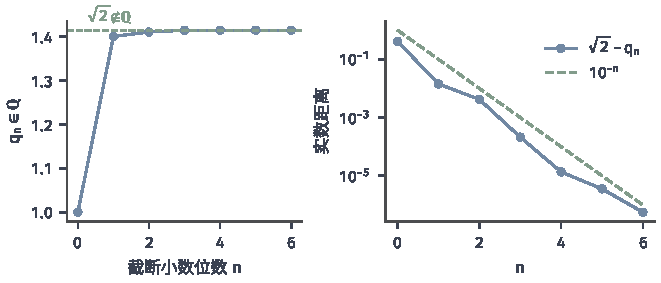
\includegraphics[width=112mm]{figures/01-mathematical-preliminaries-upper/01-mathematical-language-combinatorics-analysis-optimization/matplotlib/comprehension-additions/cauchy-completeness.pdf}
  \caption{令$q_n=\lfloor10^n\sqrt2\rfloor/10^n$，展示$n=0,\ldots,6$。左图各项均为有理数，虚线是实数极限$\sqrt2$；右图的实数距离满足$0<\sqrt2-q_n<10^{-n}$，用对数纵轴显示。有限个点不代替柯西性证明；该误差界与三角不等式才控制任意两个尾部项。}
  \label{fig:vol1-add-cauchy-completeness}
\end{figure}

\paragraph{闭集中的极限保留}

收敛与完备性保证逼近有终点后，还要检查终点是否仍满足原来的范围约束。前面用补集为开定义闭集，下面把这一条件改写为序列极限的保留条件。

\begin{lemma}[闭集的序列判据]
\label{lem:analysis-closed-sequence-criterion}
设$C$为度量空间$X$的子集。$C$闭当且仅当：对每个由$C$中点组成的序列，
若$x_n\to x$在$X$中成立，则$x\in C$。
\end{lemma}
\begin{proof}
若$C$闭而$x\notin C$，开集$X\setminus C$包含某个$B(x,r)$。
收敛要求充分靠后的$x_n$落入这个球，与$x_n\in C$矛盾。
反之，若$C$不闭，则存在$x\in X\setminus C$，使每个$B(x,r)$都与$C$相交。
为每个$n$选$x_n\in C\cap B(x,1/n)$，便有$x_n\to x\notin C$，违反序列条件。
\end{proof}

因此，完备度量空间的闭子集在继承的距离下也完备：子集中的柯西列先在母空间收敛，
闭性再保证极限仍在子集中。反过来，任一完备子空间在母度量空间中都是闭的，
因为在母空间收敛的子空间点列必为柯西列，子空间内的极限由唯一性等于原极限。
闭与有界描述不同性质；例如$(0,1)$有界但不闭，$\mathbb R$闭但不有界。

\subsection{输入趋近时的输出控制}
\label{sec:analysis-metric-continuity-extrema}

有了输入和输出的距离，就可以检查函数是否把接近的输入映成接近的输出。先在一个位置给出极限和连续性，再看能否为所有位置使用同一个输入精度。后两种统一控制分别由一致连续和Lipschitz条件表达。

\subsubsection{一点附近的函数变化}

\paragraph{函数极限与连续性}

对$f:X\to Y$及定义域$X$的一个聚点$a$（每个去掉$a$的邻域都含有$X$中的点），函数极限$\lim_{x\to a}f(x)=b$要求：对任意$\varepsilon>0$，存在$\delta>0$，使
\[
 0<d_X(x,a)<\delta\quad\Longrightarrow\quad d_Y(f(x),b)<\varepsilon.
\]
这里排除$x=a$，所以函数在$a$的取值甚至可以没有定义。连续性则要求$a$属于定义域，并把极限值与$f(a)$联系起来。对于定义域中的孤立点，足够小的邻域只含该点，连续性条件也自然成立。

确定输入与输出的距离后，可以要求小的输入扰动只引起小的输出扰动。这就把熟悉的
实函数连续性推广到一般度量空间。

为什么需要这项性质？因为它保证“先取极限再代入函数”与“先代入函数再取极限”结果相同。
若已知$x_n\to x$，我们希望$f(x_n)$的极限可以直接写成$f(x)$，而不必每换一列输入就
重做一次极限计算。连续映射就是允许这样做的函数；后面的隐函数定理、积分号下求导
都依赖这条替换规则。
\Needspace{12\baselineskip}
\begin{definition}[度量空间中的连续映射]
\label{def:analysis-continuity}
设$(X,d_X)$与$(Y,d_Y)$为度量空间。函数$f:X\to Y$在$x\in X$处
\term{连续}（continuous），是指
\[
  \begin{gathered}
    \forall\varepsilon>0,\quad \exists\delta>0,\quad \forall x'\in X,\\
    d_X(x,x')<\delta\Longrightarrow d_Y\bigl(f(x),f(x')\bigr)<\varepsilon.
  \end{gathered}
\]
若$f$在每个$x\in X$处连续，则称$f$在$X$上连续。
\end{definition}
这里$\delta$可以依赖所考察的位置$x$和要求的精度$\varepsilon$。在度量空间中，也可以用序列检验同一个条件：任意趋向$x$的$x_n$都使$f(x_n)$趋向$f(x)$。因此，已知$x_n\to x$且$f$在$x$处连续时，才可写成$f(\lim_nx_n)=\lim_nf(x_n)$；两端的趋近分别使用输入和输出空间的度量。

例如恒等映射$F(x)=x$从$(\mathbb R,d_1)$映到$(\mathbb R,d_2)$时处处不连续。
在任意$x$附近，总能找到通常距离任意小但不等于$x$的$x'$，它们的输出距离却始终为
$1$，无法小于$\varepsilon=1/2$。反过来，从$(\mathbb R,d_2)$到
$(\mathbb R,d_1)$的同一公式连续：选$\delta=1/2$，输入距离小于$\delta$就只可能
有$x'=x$，输出距离于是为$0$。这不是函数公式发生变化，而是输入输出空间对
“附近”的判断不同。图~\ref{fig:analysis-metric-convergence}右侧显示前一种失败。

\begin{figure*}[htbp]
  \centering
  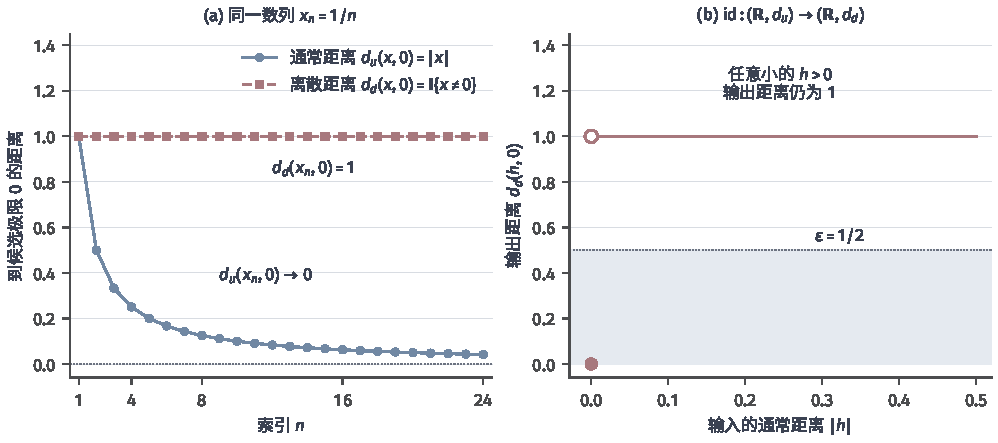
\includegraphics[width=169.0mm]{figures/01-mathematical-preliminaries-upper/01-mathematical-language-combinatorics-analysis-optimization/matplotlib/analysis-metric-convergence/figure.pdf}
  \caption{数值相同，距离不同。图中$d_u,d_d$分别对应正文的通常距离$d_1$与离散距离$d_2$。（a）数列 $x_n=1/n$ 到 $0$ 的通常距离趋于零，离散距离却恒为 $1$，所以收敛要连同度量说明。（b）恒等映射从通常度量空间映入离散度量空间时，任意非零且很小的输入位移仍对应输出距离 $1$，不能进入 $\varepsilon=1/2$ 的输出邻域，故它在 $0$ 处不连续。图为解析教学示例。}
  \label{fig:analysis-metric-convergence}
\end{figure*}

\paragraph{连续运算与函数复合}

连续性可以沿已有的计算关系传递。若$f,g:X\to\mathbb R$在$a$处连续，和、积都在$a$处连续；商还要求$g(a)\neq0$，连续性随后保证分母在一个邻域内不为零。若$f:X\to Y$在$a$处连续，$G:Y\to Z$在$f(a)$处连续，则$G\circ f$在$a$处连续。给定输出误差，先从$G$取得中间量的误差阈值，再从$f$取得输入阈值，就得到复合映射的控制。

这些规则建立在同一个位置的极限之上，不能跨过定义域限制。例如$1/x$在每个非零位置连续，却不能据此为$0$指定一个连续延拓；$|x|$处处连续，也仍需另查原点处是否存在共同斜率。

\subsubsection{整个范围上的变化控制}

\paragraph{一致连续的共同误差半径}

一个直观的图像是：普通连续只要求每个点周围都有一小片区域映射得足够近，但这片区域在陡峭处
可以缩得极小；一致连续则要求存在一个统一大小的“近邻半径”，在定义域任何位置都管用。
若要在事先不知道具体位置的情况下选一个输入误差阈值，并用它统一控制整个定义域的输出
误差，就需要让$\delta$不依赖位置。这一更强要求称为一致连续；它使同一个输入精度
足以控制整个定义域上的输出误差，因此可用于后面某些统一近似的证明。
它与函数列的一致收敛约束的对象不同：前者比较同一个函数在两个位置的值，后者比较
近似函数与目标函数在同一位置的值，不要求这些函数先一致连续。
\begin{definition}[一致连续映射]
\label{def:analysis-uniform-continuity}
设$(X,d_X)$与$(Y,d_Y)$为度量空间，$f:X\to Y$。若对每个$\varepsilon>0$都能找到一个与具体位置无关的$\delta>0$，使任意
$x,x'\in X$只要$d_X(x,x')<\delta$便有
$d_Y(f(x),f(x'))<\varepsilon$，就称$f$\term{一致连续}
（uniformly continuous）。
\end{definition}
连续性本身并不足以给出这种统一控制：
$f(x)=x^2$在$\mathbb{R}$上连续，令$x\to+\infty$并取$x'=x+1/x$，可见输入距离趋于零而输出距离
$|f(x')-f(x)|=2+1/x^2$不趋于零。

\paragraph{Lipschitz条件的比例控制}

一致连续给出统一的输入阈值，却没有要求输出误差与输入误差成固定比例。若还希望用一个常数直接估计误差的放大倍数，就要进一步要求线性上界。
\begin{definition}[Lipschitz连续映射]
\label{def:analysis-lipschitz-continuity}
设$(X,d_X)$与$(Y,d_Y)$为度量空间，$f:X\to Y$。若存在有限常数$L\geq0$，使所有$x,x'\in X$都满足
\begin{equation}
  d_Y\bigl(f(x),f(x')\bigr)\leq Ld_X(x,x'),
\label{eq:analysis-lipschitz-condition}
\end{equation}
则称$f$为$L$-\term{Lipschitz连续}（Lipschitz continuous）。
\end{definition}
当$L>0$时，取$\delta=\varepsilon/L$便得到一致连续性；$L=0$时函数为常值，也一致连续。
函数$f(x)=\sqrt{x}$在$[0,1]$上满足$|\sqrt{x}-\sqrt{x'}|\leq\sqrt{|x-x'|}$，
因而选$\delta=\varepsilon^2$就得到一致连续性，却不能得到Lipschitz连续性：若存在有限$L$，
令$x'=0$便会要求$\sqrt{x}\leq Lx$，即$1/\sqrt{x}\leq L$，这在$x\downarrow0$时不可能成立。
同一个公式在不同定义域上可能具有不同的统一控制。$f(x)=x^2$在$[0,1]$上满足
$|x^2-z^2|\leq2|x-z|$，因而$2$-Lipschitz；在整个实线上却没有有限的全局Lipschitz
常数。这两个例子说明，统一的$\varepsilon$--$\delta$控制与线性误差上界仍是不同要求。

\term{局部Lipschitz函数}（locally Lipschitz function）要求每个点附近的函数变化
都能由某个有限Lipschitz常数控制。与全局Lipschitz条件不同，各个邻域可以使用不同的常数。
\begin{definition}[局部Lipschitz函数]
\label{def:analysis-local-lipschitz}
设$U\subseteq\mathbb{R}^d$为开集，$f:U\to\mathbb{R}$。若对每个$\bm{x}\in U$，
都存在半径$r>0$与有限常数$L\geq0$，使$B(\bm{x},r)\subseteq U$，并且
\[
  |f(\bm{y})-f(\bm{z})|
  \leq L\lVert\bm{y}-\bm{z}\rVert_2
  \quad\text{对所有 }\bm{y},\bm{z}\in B(\bm{x},r)\text{成立},
\]
则称$f$在$U$上局部Lipschitz。
\end{definition}

这里$r$与$L$可以依赖中心点；一旦邻域确定，同一个$L$须控制其中的任意两点。
例如$f(x)=x^2$在任意$(x_0-r,x_0+r)$上可取$L=2(|x_0|+r)$，所以在实轴上
局部Lipschitz，却不是全局Lipschitz。向量值函数也用输出范数替换绝对值，
作完全相同的局部定义。局部控制要提升为区域内的统一控制，还需要区域或导数的额外条件。

\subsection{定义域限制下的统一控制与极值达到}

前面只规定函数的变化条件。现在把定义域也纳入判断：近似最优点可能逃向无穷远，或趋向被排除的边界。紧致性用于从序列中保留域内的极限子列；再与连续性结合，才得到极值达到和共同的误差尺度。

\subsubsection{有界序列能否保留收敛子列}

\paragraph{紧致性与有限覆盖}

第~\ref{chap:sets-functions-and-proofs}章已区分下确界与最小值：数值可以逼近一个下界，却始终找不到达到它的点。
要让近似最优点最终提供一个可行解，需要防止点列逃向无穷远或被排除的边界。
在一般度量空间中，承担这一职责的是紧致性。可以用一个最优化的直觉理解它：要在一列越来越好
的候选里取出真正的极限点，定义域必须是“封闭且走不出去”的，否则逼近序列可能收敛到定义域
边界外的点，那个点又恰好是最优值所在。紧致性正是这种“任何逼近序列都在域内留下聚点”的
保证。它并不保证函数有下界，只保证定义域本身
不留“逼近点可以逃出去”的缺口；配合连续性才能把下确界转成最小值。
\begin{definition}[开覆盖与紧致性]
\label{def:analysis-compactness}
设$(X,d)$为度量空间，$K\subseteq X$。若一族$X$中的开集的并包含$K$，就称这族开集为$K$的
\term{开覆盖}（open cover）；若从中选出的有限个开集仍覆盖$K$，它们就构成
\term{有限子覆盖}（finite subcover）。集合$K$的每个开覆盖都能选出有限子覆盖时，
称$K$为\term{紧致}（compact）。
\end{definition}
在度量空间中，这一定义等价于
\term{序列紧致性}：集合中的每个序列都有一个子序列收敛到仍在该集合中的点。
后一种表述更适合分析算法产生的点列，因为它直接提供候选极限。
我们先看开覆盖条件怎样保证这样的子列。若某个点列没有收敛子列，则对每个$x\in K$，
必有一个开球只含点列的有限项；否则可从$B(x,1/k)$中依次选取下标递增的项，构成趋于$x$的子列。
这些开球覆盖$K$，紧致性让我们选出有限个球覆盖$K$，于是整条点列也只能有有限项，矛盾。
这说明了当前需要的“开覆盖紧致$\Rightarrow$序列紧致”方向；反向等价在此不展开证明。

\paragraph{有限维中的闭且有界}

在有限维欧氏空间$\mathbb{R}^d$中，Heine--Borel定理说明紧致等价于闭且有界。这个结论不能原样搬到一般度量空间。考虑所有有界实数序列组成的空间
\[   \ell^\infty   =   \left\{\bm{x}=(x_1,x_2,\ldots):   \sup_{k\geq1}|x_k|<\infty\right\},   \qquad   d(\bm{x},\bm{y})=\sup_{k\geq1}|x_k-y_k|. \]
令$\bm{e}_n$只有第$n$个坐标为$1$，其余坐标为$0$。集合$\{\bm{e}_n:n\geq1\}$有界，且不同元素的距离恒为$1$。因此由该集合中元素组成的收敛点列必最终常值：柯西条件取误差$1/2$后，尾部不能再含两个不同元素。极限仍在集合内，由闭集的序列判据可知它闭。然而原点列$(\bm e_n)$的任何子序列都不是柯西数列，更不可能收敛。一般空间中 “闭且有界”不足以替代紧致，正是因为无穷多个彼此分离的方向可能留在同一个有界球内。

\subsubsection{连续函数能否达到极值}

\paragraph{极值达到的条件}

定义域能保留极限子列，还需让函数值随这些点连续变化，才能把近似极值变成实际达到的值。紧致性与连续性在下面分别承担这两项职责。

\begin{theorem}[紧致集上的极值定理]
\label{thm:analysis-extreme-value}
设$K$是非空紧致度量空间，$f:K\to\mathbb{R}$连续，则$f$在$K$上同时达到最小值与最大值。
\end{theorem}
这里回顾熟悉的极值定理，不再展开证明。紧致性的两项作用是从近似最优点列中抽出收敛子序列，并保证极限仍在可行集合内。连续性随后把函数值极限传到该点。任一条件缺失都可能使最优解不存在。
\begin{example}[极值存在条件怎样失效]
\label{ex:analysis-extrema-failures}
在开区间$(0,1)$上，连续函数$f(x)=x$的下确界为$0$，却没有最小点；定义域不紧致， 极限点$0$被排除。把定义域改成闭但不紧致的$\mathbb{R}$，连续函数$f(x)=e^x$仍有下确界$0$而不达到它。另一方面，在紧致集合$[0,1]$上定义
\[   g(0)=1,\qquad g(x)=x\quad(x>0), \]
则$\inf g=0$也未达到；这次失败的是$g$在$0$处不连续。三个例子分别表明“连续”、 “闭”或“有界”中的单独一项都不是一般的极值存在保证。
\end{example}

连续性控制函数值，不直接控制斜率。对一元函数，导数还要求左右两侧的差商趋向同一个值：$x^2$在$0$同时满足这两项要求，$|x|$的函数值趋向$0$却有两个不同的侧向斜率，阈值函数$\mathbb I\{x\geq0\}$则连左右函数值都不趋向同一个数。
尖点只阻止共同斜率，跳跃连共同的函数值极限也破坏了。
图~\ref{fig:analysis-continuity-counterexamples}把三者放在同一位置比较；
下一小节将写出差商和整体线性近似的正式条件。

\begin{figure*}[htbp]
  \centering
  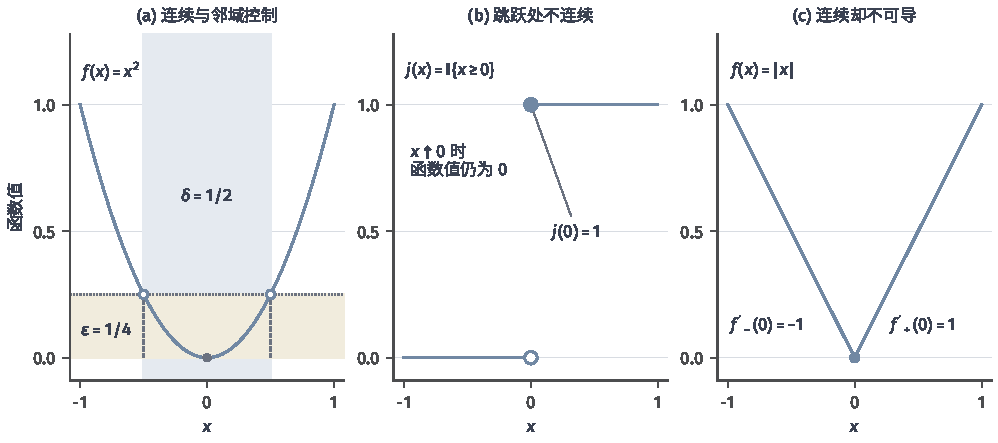
\includegraphics[width=169.0mm]{figures/01-mathematical-preliminaries-upper/01-mathematical-language-combinatorics-analysis-optimization/matplotlib/analysis-continuity-counterexamples/figure.pdf}
  \caption{三个不同的局部性质。（a）$f(x)=x^2$ 在 $0$ 处可用 $\delta=1/2$ 控制 $\varepsilon=1/4$：严格位于输入邻域内的点，其函数值严格落在输出邻域内。（b）阶跃函数在 $0$ 的左极限为 $0$，取值却为 $1$，空心点和实心点区分两者。（c）$|x|$ 在 $0$ 处连续，但左右导数分别为 $-1$ 和 $1$，不存在共同的双侧导数。图中曲线均为解析教学示例。}
  \label{fig:analysis-continuity-counterexamples}
\end{figure*}

\paragraph{紧致范围上的一致连续}

紧致性还能把逐点连续提升为一致连续：连续映射在紧致定义域上一定一致连续。
若它不一致连续，就能找到某个$\varepsilon_0>0$及点对$x_n,y_n\in K$，使
$d(x_n,y_n)<1/n$，而$d_Y(f(x_n),f(y_n))\geq\varepsilon_0$。
由序列紧致性选出$x_{n_k}\to x\in K$，三角不等式又给出$y_{n_k}\to x$。
连续性使两列函数值都趋于$f(x)$，与输出距离下界矛盾。
这为前面闭区间上的统一控制提供了一个一般条件，但不保证Lipschitz连续；
$\sqrt{x}$的例子已说明，输出变化未必能由输入距离的一次常数倍控制。

\section{函数的微分与局部近似}
\label{sec:analysis-local-models}

连续性保证输入变化足够小时输出变化也小，但没有说明变化沿什么方向、按什么比例发生。微分用局部线性或高阶模型回答这些问题。下面先建立变化的表示，再研究变化怎样沿复合计算、矩阵运算和隐式方程传递，最后控制有限位移与截断误差。尖点处的失效用方向差商说明，正式广义梯度放到第~\ref{chap:measurable-functions}章。

\subsection{局部变化的表示}
\label{sec:analysis-derivatives-linear-approximation}

在$f(x)=x^2$中，一个小输入增量可以分成线性响应和更小的余项；多元函数则要求所有小扰动共享一个线性响应。由此建立导数、全微分和Jacobian，再用Hessian描述线性响应怎样改变。对于绝对值的尖点，共同线性响应不存在，需要保留方向信息。

\subsubsection{一阶变化的线性表示}

\paragraph{差商、方向导数与偏导数}

从一元函数开始，把输出增量除以输入增量，得到这一小段上的平均变化率；
输入增量趋零后若仍有稳定值，就用它预测附近的输出。只保留一段的话，平均变化率会随
所取区间改变；使这个比值在区间长度趋零时有唯一极限，就把“局部斜率”从一个区间上的
平均值变成该点自身的性质。

一元函数$f:\mathbb{R}\to\mathbb{R}$在$x$处的\term{导数}（derivative）定义为
\[   f'(x)=\lim_{h\to0}\frac{f(x+h)-f(x)}{h}, \]
前提是这个双侧极限存在。
用一个具体数字体会它预测什么。取$f(x)=x^2$、$x=3$，在$h=0.1$时真实增量是
$3.1^2-3^2=0.61$，而用该点斜率$6$预测的一阶增量是$6\times0.1=0.6$，误差仅$0.01$；
$h$越小，这个相对误差越小。导数正是把“这一小段平均每单位输入变化引起多少输出变化”
在段长趋于零时的稳定值提取出来。
它说明输入发生小变化$h$时，函数增量的一阶部分是$f'(x)h$：
\begin{equation}
  f(x+h)=f(x)+f'(x)h+o(|h|).
\label{eq:analysis-scalar-first-order}
\end{equation}
第~\ref{sec:comb-growth-scales}节的小$o$仍表示相对余项趋零，不过这里的趋向是$h\to0$：余项$r(h)$满足$r(h)/|h|\to0$，不只是$h$本身很小。导数存在必然推出函数在该点连续，但连续不保证可导，例如$|x|$在$0$处连续，左右导数却分别为 $-1$和$1$。
这也解释了图中尖点与跳跃的区别；两者都不能使用经典双侧导数，失效的层次却不同。

对$f:\mathbb{R}^d\to\mathbb{R}$，沿方向$\bm{v}\in\mathbb{R}^d$的
\term{方向导数}（directional derivative）是
\[   D_{\bm{v}}f(\bm{x})   =   \lim_{t\to0}   \frac{f(\bm{x}+t\bm{v})-f(\bm{x})}{t}. \]
取$\bm{v}$为第$j$个坐标方向$\bm{e}_j$，就得到\term{偏导数}
（partial derivative）$\partial f/\partial x_j$。方向导数只检查一条直线，而整体可微性要求所有小扰动共享同一个线性近似。

\paragraph{全微分与Jacobian}

所有方向共享的近似还必须与扰动的叠加和缩放相容：把扰动写成
$\alpha\bm u+\beta\bm v$时，预测增量也应为两部分预测增量的同样组合。
满足
\[
 A(\alpha\bm u+\beta\bm v)=\alpha A(\bm u)+\beta A(\bm v)
 \quad(\bm u,\bm v\in\mathbb R^d,\ \alpha,\beta\in\mathbb R)
\]
的映射称为线性映射。例如固定向量$\bm a$后，$A(\bm h)=\bm a^\top\bm h$
把每个坐标的扰动乘以固定系数再相加。可微性要求用同一个这样的映射解释全部小扰动。

函数$f:\mathbb{R}^d\to\mathbb{R}$在$\bm{x}$处\term{可微}
（differentiable），是指存在一个线性映射 $A:\mathbb{R}^d\to\mathbb{R}$，使
\begin{equation}
  f(\bm{x}+\bm{h})
  =
  f(\bm{x})+A(\bm{h})+o(\lVert\bm{h}\rVert_2).
\label{eq:analysis-total-differentiability}
\end{equation}
线性部分$A(\bm h)$称为全微分，也记为$\mathrm df_{\bm x}(\bm h)$。
条件要求对任意趋零的非零扰动$\bm h$都有
$|f(\bm x+\bm h)-f(\bm x)-A(\bm h)|/\lVert\bm h\rVert_2\to0$，
而不是先固定一个方向，再允许误差控制随方向改变。
在欧氏空间中，每个这样的线性泛函都可写为 $A(\bm{h})=\langle\nabla f(\bm{x}),\bm{h}\rangle$，其中
\[   \nabla f(\bm{x})   =   \left(     \frac{\partial f}{\partial x_1}(\bm{x}),\ldots,     \frac{\partial f}{\partial x_d}(\bm{x})   \right)^{\top} \]
称为\term{梯度}（gradient）。因此梯度不是若干偏导数的随意排列，而是表示局部线性映射的向量；扰动$\bm{h}$通过内积变成函数的一阶变化。

可微必然推出所有方向导数存在，并且 $D_{\bm{v}}f(\bm{x})=\langle\nabla f(\bm{x}),\bm{v}\rangle$。反向结论不成立， 仅有偏导数更不够。
\begin{example}[偏导数存在但不可微]
\label{ex:analysis-partials-not-differentiable}
定义$f:\mathbb{R}^2\to\mathbb{R}$为
\[   f(x,y)=
\begin{cases}     \dfrac{xy}{\sqrt{x^2+y^2}}, & (x,y)\neq(0,0),\\[6pt]     0, & (x,y)=(0,0).
\end{cases} \]
沿两条坐标轴，函数恒为$0$，所以 $\partial f/\partial x(0,0)=\partial f/\partial y(0,0)=0$。若$f$在原点可微， 候选线性部分只能是零映射。可是沿$\bm{h}=(t,t)$，
\[   \frac{|f(t,t)-f(0,0)|}{\lVert(t,t)\rVert_2}   =   \frac{|t|/\sqrt{2}}{\sqrt{2}|t|}   =\frac12, \]
余项与$\lVert\bm{h}\rVert_2$之比不趋于零，故$f$在原点不可微。偏导数只看坐标轴，遗漏了其他接近路径。本例沿每个方向$\bm v=(a,b)$的
正向方向导数都存在，这里只令$t\downarrow0$，得到$ab/\sqrt{a^2+b^2}$（零方向取$0$）；它却不是关于$\bm v$
的线性函数，而且双侧方向导数在$ab\neq0$时不存在。方向极限采用单侧还是双侧，
必须与所用定义一致；本节定义采用双侧极限。
\end{example}

一个常用的充分条件是：若$f$的所有一阶偏导数在$\bm{x}$的某个邻域内存在，并在 $\bm{x}$处连续，则$f$在$\bm{x}$处可微。注意这只是方便核对的充分条件，不是必要条件； 可微函数的偏导数不一定在该点附近连续。

即使每个双侧方向导数都存在，也未必可微。例如令
$g(x,y)=x^3/(x^2+y^2)$于非零点，$g(0,0)=0$。
沿$\bm v=(a,b)\neq\bm0$有$D_{\bm v}g(0,0)=a^3/(a^2+b^2)$，
但坐标方向导数给出的候选梯度为$(1,0)^\top$，它对方向$(1,1)^\top$
预测$1$而非实际的$1/2$。这些方向变化率无法拼成一个线性映射。
与前例的单侧方向极限相比，这里直接检验了本节采用的双侧定义。

用$f(x)=x^3-3x$保留一个贯穿例子。在$x_0=1/2$处，
\[
  f(x_0)=-\frac{11}{8},\qquad f'(x_0)=3x_0^2-3=-\frac94.
\]
输入改变$h$时，一阶近似给出
\begin{equation}
  T_1(h)=f(x_0)+f'(x_0)h=-\frac{11}{8}-\frac94h.
\label{eq:analysis-cubic-linear-model}
\end{equation}
取$h=0.1$，$T_1(h)=-1.600$，而实际$f(0.6)=-1.584$。近似抓住了下降方向和主要
变化量，但还有$0.016$的误差；第~\ref{sec:analysis-second-order-curvature}节将用曲率解释这部分差别。

当一个输入产生多个输出时，每个输出都有一行局部线性系数，把这些行排在一起便得到
Jacobian矩阵。复合计算只需再把前一层的输出扰动作为后一层的输入扰动。
设$f:\mathbb{R}^d\to\mathbb{R}^m$。若存在矩阵 $\bm{J}_f(\bm{x})\in\mathbb{R}^{m\times d}$使
\begin{equation}
  f(\bm{x}+\bm{h})
  =
  f(\bm{x})+\bm{J}_f(\bm{x})\bm{h}
  +o(\lVert\bm{h}\rVert_2),
\label{eq:analysis-jacobian-linearization}
\end{equation}
则称$f$在$\bm{x}$处可微，$\bm{J}_f(\bm{x})$称为
\term{Jacobian矩阵}（Jacobian matrix）。其第$i,j$个元素是 $\partial f_i/\partial x_j$。矩阵有$m$行、$d$列，因为它把$d$维输入扰动映射成 $m$维输出扰动。

\subsubsection{二阶变化的曲率表示}
\label{sec:analysis-second-order-curvature}

\paragraph{Hessian与方向曲率}

上一节的线性近似在$x_0=1/2$处把函数值预测为$-1.600$，实际为$-1.584$，偏差$0.016$。
这个偏差从哪里来？因为斜率本身也在随位置改变。要估计这个偏差，就要知道斜率沿每个方向
改变得多快，这需要比一阶导数更高一阶的信息。

延续$f(x)=x^3-3x$的例子，一阶导数$f'(x)=3x^2-3$还随位置变化。再求一次导数，
得到$f''(x)=6x$，所以$f''(1/2)=3$。在$x_0=1/2$附近，斜率向右移动时增大，
曲线向上弯；这解释了真实值为何高于前节的切线预测。图~\ref{fig:analysis-derivative-orders}将切线和下面的二次修正放在同一幅曲线图上比较。加入二次项得到
\begin{equation}
  T_2(h)=T_1(h)+\frac12f''(x_0)h^2
        =-\frac{11}{8}-\frac94h+\frac32h^2.
\label{eq:analysis-cubic-quadratic-model}
\end{equation}
在$h=0.1$时，$T_2=-1.585$，与实际值$-1.584$只差$0.001$。
一阶导数回答此处沿给定方向增还是减，二阶导数回答这个变化率怎样改变。
第~\ref{sec:analysis-taylor-approximation}节将用Taylor展开给出一阶和二阶余项的完整表达式。

一阶近似只保留函数的局部斜率。若还要判断这个斜率怎样随位置改变，就需要
\term{Hessian矩阵}（Hessian matrix）。设$f:\mathbb{R}^d\to\mathbb{R}$在 $\bm{x}$附近二阶可微，定义
\[   \nabla^2 f(\bm{x})   =
\begin{bmatrix}     \dfrac{\partial^2 f}{\partial x_1^2} &     \cdots &     \dfrac{\partial^2 f}{\partial x_1\partial x_d}\\     \vdots & \ddots & \vdots\\     \dfrac{\partial^2 f}{\partial x_d\partial x_1} &     \cdots &     \dfrac{\partial^2 f}{\partial x_d^2}
\end{bmatrix}. \]
若二阶偏导数在邻域内连续，混合偏导数可以交换，Hessian矩阵因而对称。
这里把方表$\bm H$与方向$\bm v$组合而成的二次表达式
$\bm v^\top\bm H\bm v=\sum_{i=1}^d\sum_{j=1}^d H_{i,j}v_i v_j$称为二次型。
对方向$\bm v$，$\bm{v}^{\top}\nabla^2f(\bm{x})\bm{v}$是沿直线
$t\mapsto f(\bm{x}+t\bm{v})$在$t=0$处的二阶导数。它衡量的是沿该方向的一阶斜率变化。

对二次函数
\[   f(\bm{x})   =   \frac12\bm{x}^{\top}\bm{A}\bm{x}   +\bm{b}^{\top}\bm{x}+c, \]
只有$\bm{A}$的对称部分影响函数值。令 $\bm{H}=(\bm{A}+\bm{A}^{\top})/2$，则 $\nabla f(\bm{x})=\bm{H}\bm{x}+\bm{b}$且 $\nabla^2f(\bm{x})=\bm{H}$。
例如$\bm H=\operatorname{diag}(2,100)$时，方向二次型为$2v_1^2+100v_2^2$，
沿两个坐标方向都向上弯，但第二个方向的二阶变化率是第一个的$50$倍。
若改为$\operatorname{diag}(2,-100)$，两个坐标方向的弯曲方向便相反。
判断曲率需要检查整个二次型，而不是某一个对角元素。

对实对称矩阵$\bm H$，若每个非零$\bm v$都有$\bm v^\top\bm H\bm v>0$，称$\bm H$正定；
若只要求$\bm v^\top\bm H\bm v\geq0$，则称半正定。
把不等号反向得到负定与半负定；若既存在使二次型为正的方向，又存在使它为负的方向，
则称矩阵不定。这些名称分别说明全部方向或某些方向上的曲率符号。

\paragraph{驻点附近的局部形状}

函数在当前点附近是增是减，可用于判断局部极值。局部极小点是指某个邻域内
所有函数值都不小于该点的值；严格局部极小还要求其他点的值严格更大。
设$\bm{x}^{\star}$是开集内部的局部极小点，且$f$在该点可微。对每个方向 $\bm{v}$考察$f(\bm{x}^{\star}+t\bm{v})$，一元函数的必要条件给出 $\nabla f(\bm{x}^{\star})^{\top}\bm{v}=0$。这对所有$\bm{v}$成立，因此
\begin{equation}
  \nabla f(\bm{x}^{\star})=\bm{0}.
\label{eq:analysis-first-order-necessary}
\end{equation}
若$f$还在该点二阶可微，同样沿任意方向使用一元二阶必要条件，可得
\begin{equation}
  \bm{v}^{\top}\nabla^2f(\bm{x}^{\star})\bm{v}\geq0
  \quad\text{对所有 }\bm{v},
\label{eq:analysis-second-order-necessary}
\end{equation}
即Hessian矩阵半正定。局部极大点对应半负定。这些只是必要条件：
$f(x)=x^4$与$f(x)=-x^4$在$0$处分别有严格局部极小值和严格局部极大值，
二者的二阶导数却都为零；$f(x)=x^3$在$0$处的一阶导数和二阶导数也都为零，
却没有极值。Hessian矩阵半正定或半负定本身不能决定驻点类型。

驻点处各方向的二阶变化都为正，即Hessian正定，并且函数在邻域内二阶连续可微时，该点是严格局部极小点；负定时对应严格局部极大点。不定时存在一增一减两个方向，形成鞍点。这里只先说明判别的含义；从局部曲率到原函数的严格判断，还需要控制高阶余项，第~\ref{sec:analysis-taylor-approximation}节将给出完整论证。

\subsubsection{不可微位置的方向变化}
\label{sec:analysis-directional-nonsmooth}

\paragraph{尖点处的单边变化}

绝对值在$0$处连续，右侧差商为$1$，左侧差商为$-1$，因此没有共同的双侧导数。若只考察从当前位置沿给定方向前进，可以令$t\downarrow0$，定义正向方向差商的极限
\[
 D^+_v f(x)=\lim_{t\downarrow0}\frac{f(x+tv)-f(x)}{t}.
\]
对$f(x)=|x|$及$x=0$，这个极限为$|v|$。它对每个方向都有值，却不满足线性性：方向$1$和$-1$都得到$1$。ReLU函数$\max\{0,x\}$在$0$处同样有正向方向导数$\max\{0,v\}$。这里采用的正向极限与前面双侧方向导数是两个约定，使用时必须写明。

\paragraph{方向信息与单一梯度的边界}

如果一个向量真能表示全微分，其与方向的内积必须同时给出所有方向的一阶变化。绝对值和ReLU的正向方向变化不满足这一要求，任意指定一个梯度值也不能使函数变得可微。第~\ref{chap:measurable-functions}章将在局部Lipschitz条件下，用附近可微位置的梯度集合描述尖点；这仍不等于在尖点恢复一个经典导数。


在含阈值或脉冲事件的模型中，常保留离散前向映射，却在反向计算时把其导数替换成某个平滑且非零的函数。这种信号称为\term{替代梯度}（surrogate gradient）。它是算法人为指定的近似更新方向，不自动等于前向映射的经典导数，也通常不满足凸次梯度的不等式。因此使用时应分别写清前向函数、反向替代函数及其尺度，不能把训练规则描述成对原离散函数的精确求导。

中心差分
\[   \frac{f(x+\varepsilon)-f(x-\varepsilon)}{2\varepsilon} \]
检验的是实际代入的函数$f$在尺度$\varepsilon$上的变化。若前向计算采用离散函数，反向计算另行指定平滑信号，差分与反向信号就对应不同对象。核验程序时，应分别检查离散前向函数是否正确，以及反向信号是否符合指定的学习规则；不能把二者相等作为未经说明的检验标准。

\subsection{函数关系中的变化传递}
\label{sec:analysis-vector-chain-matrix-calculus}

实际计算往往把多个函数连接起来，或由矩阵运算、方程关系间接决定输出。它们共享的任务是把已知的局部变化传到最终结果，但所需信息不同：复合映射直接传递Jacobian；矩阵变量要保持乘法结构；隐式关系还必须先保证存在可微解分支。

\subsubsection{复合映射中的变化传递}

\paragraph{链式法则与乘法顺序}

若一次计算的输出成为下一次计算的输入，前一映射产生的局部扰动还要再经过后一映射的线性响应。复合后的响应因此是两个Jacobian的乘积，先后次序由实际计算关系决定。

若$f$在$\bm{x}$处可微，且$g:\mathbb{R}^m\to\mathbb{R}^p$在$f(\bm{x})$处可微，则复合映射满足
\begin{equation}
  \bm{J}_{g\circ f}(\bm{x})
  =
  \bm{J}_g\bigl(f(\bm{x})\bigr)\bm{J}_f(\bm{x}).
\label{eq:analysis-vector-chain-rule}
\end{equation}
这就是\term{链式法则}（chain rule）。维度同时给出乘法次序： $(p\times m)(m\times d)=p\times d$，反向相乘往往没有定义。即使方阵$\bm A,\bm B$同阶、两个次序的乘积都有定义，也通常有$\bm A\bm B\neq\bm B\bm A$，不能据标量求导经验调换因子。

\paragraph{标量目标的反向求导}

上面的$g$允许向量输出。当$p=1$时，$g$把中间向量变成一个标量。在优化问题中，
这个标量通常是待最小化的目标值，本书便把此时的$g$记为$\ell$。令
$\bm y=f(\bm x)$，总目标就是$L(\bm x)=\ell(f(\bm x))$；$\ell$只是原复合映射的
最后一层，并没有增加一个未说明的输出。采用列向量梯度，链式法则写成
\[
  \nabla L(\bm x)
  =\bm J_f(\bm x)^\top\nabla\ell(\bm y)\big|_{\bm y=f(\bm x)}.
\]
局部线性映射在前向计算中按$\bm J_f$作用，在标量目标的反向计算中按转置
$\bm J_f^\top$传回。这是后续反向传播的线性代数核心，具体网络结构留到模型章节。

\begin{example}[从中间向量求回复合目标的梯度]
\label{ex:analysis-chain-rule-calculation}
令
\[
  f(x_1,x_2)=(x_1^2,x_1x_2,x_2)^\top,
  \qquad \ell(\bm y)=\frac12(y_1^2+y_2^2+y_3^2).
\]
$f$从二维输入产生三维中间量，$\ell$再把三维中间量变成一个数。于是
\[
  \bm J_f=\begin{bmatrix}2x_1&0\\x_2&x_1\\0&1\end{bmatrix},
  \qquad \nabla\ell(\bm y)=\bm y.
\]
在$\bm x=(1,2)^\top$处，$\bm y=(1,2,2)^\top$，链式法则给出
\[
  \nabla L(1,2)
  =\begin{bmatrix}2&2&0\\0&1&1\end{bmatrix}
    \begin{bmatrix}1\\2\\2\end{bmatrix}
  =\begin{bmatrix}6\\4\end{bmatrix}.
\]
也可以把复合函数直接展开为
$L(x_1,x_2)=\tfrac12(x_1^4+x_1^2x_2^2+x_2^2)$，求偏导得到
$\nabla L=(2x_1^3+x_1x_2^2,\,x_1^2x_2+x_2)^\top$，在同一点仍为$(6,4)^\top$。
两种计算处理同一个目标；链式形式保留了中间映射，可分别复用各层的导数。
矩阵形状$(2\times3)(3\times1)=2\times1$也核对了梯度传递的次序。
\end{example}

若要把任意实数评分变成正数且总和为$1$的权重，可以先取指数再除以共同的总和。
这就是$n$维\term{归一化指数映射}（softmax）。对正整数$n$和
$\bm{z}\in\mathbb{R}^n$，令
\[
  s_i(\bm{z})
  =
  \frac{e^{z_i}}{\sum_{k=1}^n e^{z_k}},
  \qquad i=1,\ldots,n.
\]
记分母为$Z=\sum_k e^{z_k}$。指数函数求导和商法则给出
\[
  \frac{\partial s_i}{\partial z_j}
  =
  \frac{\mathbb{I}\{i=j\}e^{z_i}Z-e^{z_i}e^{z_j}}{Z^2}
  =
  s_i\bigl(\mathbb{I}\{i=j\}-s_j\bigr).
\]
因此整个Jacobian矩阵为
\begin{equation}
  \bm{J}_{\bm{s}}(\bm{z})
  =
  \operatorname{diag}(\bm{s})-\bm{s}\bm{s}^{\top}.
\label{eq:analysis-softmax-jacobian}
\end{equation}
对角项$s_i(1-s_i)$描述提高$z_i$对自身分量的影响，非对角项$-s_is_j$
来自共同分母：提高一个坐标会压低其余归一化分量。每行元素之和为零，
这也与给所有$z_i$同时加同一常数不改变输出相符。

\subsubsection{矩阵运算中的变化传递}

\paragraph{矩阵微分与迹内积}

第~\ref{chap:sets-functions-and-proofs}章已经建立矩阵乘法和转置。以下还用到逆矩阵、迹与行列式：逆矩阵$\bm X^{-1}$满足$\bm X\bm X^{-1}=\bm X^{-1}\bm X=\bm I$；对$d$阶方阵，行列式是$\det\bm X=\sum_{\pi\in S_d}\operatorname{sgn}(\pi)\prod_iX_{i,\pi(i)}$，其中$S_d$为排列集合，符号由排列的奇偶性决定。它为零恰好表示矩阵不可逆。这里采用这些有限维代数事实，系统推导见第~\ref{chap:linear-algebra}章。后面的迹内积和乘积展开会直接说明所需微分，不要求提前掌握整章线性代数。

如果输入本身是矩阵，逐条写出$mn$个偏导数会掩盖原有的矩阵乘法结构。矩阵$\bm{X}\in\mathbb{R}^{m\times n}$可以看成$mn$个坐标组成的对象，矩阵梯度则把这些一阶变化重新排回原来的形状。先固定Frobenius迹内积
\[   \langle\bm{A},\bm{B}\rangle_F   =   \operatorname{tr}(\bm{A}^{\top}\bm{B}) \]
其中$\operatorname{tr}$是方阵对角元素之和，所以这个内积也等于
$\sum_{i,j}\bm A_{i,j}\bm B_{i,j}$，对应范数为
$\lVert\bm H\rVert_F=(\sum_{i,j}\bm H_{i,j}^2)^{1/2}$。
对标量函数$f(\bm X)$，全微分要求
$f(\bm X+\bm H)=f(\bm X)+\mathrm df_{\bm X}(\bm H)+o(\lVert\bm H\rVert_F)$。
用这个内积
定义矩阵梯度：若一阶全微分能够写成
\begin{equation}
  \mathrm{d}f
  =
  \langle\nabla_{\bm{X}}f,\mathrm{d}\bm{X}\rangle_F
  =
  \operatorname{tr}\bigl((\nabla_{\bm{X}}f)^{\top}
  \mathrm{d}\bm{X}\bigr),
\label{eq:analysis-matrix-gradient-definition}
\end{equation}
则$\nabla_{\bm{X}}f$与$\bm{X}$形状相同。计算时可先用乘积法则展开微分，再利用
\[   \operatorname{tr}(\bm{A}\bm{B})   =\operatorname{tr}(\bm{B}\bm{A}),\qquad   \operatorname{tr}(\bm{A}\bm{B}\bm{C})   =\operatorname{tr}(\bm{B}\bm{C}\bm{A}), \]
把$\mathrm{d}\bm{X}$移动到末端。迹只允许循环移位，不能任意交换相邻矩阵。

先考虑二次型$q(\bm{x})=\bm{x}^{\top}\bm{A}\bm{x}$，其中 $\bm{A}\in\mathbb{R}^{d\times d}$固定。由乘积法则，
\begin{align*}
  \mathrm{d}q
  &=
  (\mathrm{d}\bm{x})^{\top}\bm{A}\bm{x}
  +\bm{x}^{\top}\bm{A}\,\mathrm{d}\bm{x}\\
  &=
  \bm{x}^{\top}(\bm{A}^{\top}+\bm{A})\,\mathrm{d}\bm{x}.
\end{align*}
因此
\begin{equation}
  \nabla_{\bm{x}}
  \bigl(\bm{x}^{\top}\bm{A}\bm{x}\bigr)
  =
  (\bm{A}+\bm{A}^{\top})\bm{x}.
\label{eq:analysis-quadratic-form-gradient}
\end{equation}
只有当$\bm{A}$对称时才能化为$2\bm{A}\bm{x}$。直接写成$2\bm{A}\bm{x}$会悄然加入对称性条件。

对固定的$\bm{A}\in\mathbb{R}^{m\times n}$，令 $f(\bm{X})=\operatorname{tr}(\bm{A}^{\top}\bm{X})$。它的微分已经符合式
\eqref{eq:analysis-matrix-gradient-definition}，所以
\begin{equation}
  \nabla_{\bm{X}}\operatorname{tr}(\bm{A}^{\top}\bm{X})
  =\bm{A}.
\label{eq:analysis-trace-linear-gradient}
\end{equation}
这个简单关系常用于从迹表达式中读出梯度。

\paragraph{逆矩阵与行列式的变化}

若方阵$\bm{X}$可逆，由恒等式$\bm{X}\bm{X}^{-1}=\bm{I}$取微分可得
\[   (\mathrm{d}\bm{X})\bm{X}^{-1}   +\bm{X}\,\mathrm{d}(\bm{X}^{-1})=\bm{0}. \]
左乘$\bm{X}^{-1}$后得到
\begin{equation}
  \mathrm{d}(\bm{X}^{-1})
  =
  -\bm{X}^{-1}(\mathrm{d}\bm{X})\bm{X}^{-1}.
\label{eq:analysis-inverse-differential}
\end{equation}
两个$\bm{X}^{-1}$位于扰动两侧，不能合并成 $-\bm{X}^{-2}\mathrm{d}\bm{X}$，因为$\mathrm{d}\bm{X}$未必与$\bm{X}^{-1}$交换。

最后设$\bm{X}\in\mathbb{R}^{d\times d}$可逆且$\det\bm{X}>0$，使实值函数$\log\det\bm{X}$有定义。
计算它的一阶变化，先把方向扰动$\bm H$从行列式中分离出来：
\[
 \det(\bm X+t\bm H)=\det(\bm X)\det(\bm I+t\bm X^{-1}\bm H).
\]
对固定矩阵$\bm B$，行列式的排列展开给出
$\det(\bm I+t\bm B)=1+t\operatorname{tr}(\bm B)+O(t^2)$。
其中一次项只能从恒等排列的一个对角位置选取$tB_{i,i}$，其余位置选$1$；
非恒等排列至少改变两个位置，因此只贡献二次及以上项。
代入$\bm B=\bm X^{-1}\bm H$，便得到Jacobi行列式公式的一阶形式
\[   \mathrm{d}\det\bm{X}   =   \det(\bm{X})\operatorname{tr}   (\bm{X}^{-1}\mathrm{d}\bm{X}). \]
再应用标量对数的链式法则，
\begin{equation}
  \mathrm{d}\log\det\bm{X}
  =
  \operatorname{tr}(\bm{X}^{-1}\mathrm{d}\bm{X}),
  \qquad
  \nabla_{\bm{X}}\log\det\bm{X}
  =
  \bm{X}^{-\top}.
\label{eq:analysis-logdet-gradient}
\end{equation}
若$\bm X$还对称，则$\bm{X}^{-\top}=\bm{X}^{-1}$；一般情形应保留转置。
这些计算都先找出扰动的一阶项，再用迹内积读出梯度；乘积次序与行列式展开决定了哪些变形成立。
\begin{example}[逆矩阵微分中的乘法次序]
\label{ex:analysis-noncommuting-inverse-differential}
取$\bm X=\operatorname{diag}(2,1)$，扰动方向
$\bm E=\begin{bmatrix}0&1\\1&0\end{bmatrix}$。沿$\bm X+t\bm E$求逆矩阵的导数为
\[
 -\bm X^{-1}\bm E\bm X^{-1}
 =\begin{bmatrix}0&-1/2\\-1/2&0\end{bmatrix}.
\]
若照搬标量规则而写成$-\bm X^{-2}\bm E$，会得到
$\begin{bmatrix}0&-1/4\\-1&0\end{bmatrix}$，连对称性都丢失。
原路径在$0$附近由对称可逆矩阵组成，其逆与导数也应对称；这一结构检查能直接发现错误。
矩阵变量沿给定方向微分时，夹在两侧的逆矩阵不能随意移到同一侧。
\end{example}

\subsubsection{隐式方程中的变化传递}
\label{sec:analysis-implicit-parameter-integral}

\paragraph{局部解分支的存在条件}

显式函数给出了每个输入对应的输出，方程$F(\bm x,\bm y)=\bm0$却只规定两者必须满足的关系。
这类关系在优化里反复出现。把一组可变化的观测数值记为$\bm\theta$，参数为$\bm w$，
目标写成$J(\bm w,\bm\theta)$；驻点方程$\nabla_{\bm w}J(\bm w,\bm\theta)=\bm0$
规定了两者的关系，却没有直接给出$\bm w$关于$\bm\theta$的公式。
想知道观测数值微调后驻点怎样移动，需要先固定一个驻点，再确认方程在它附近确定
唯一且可微的分支。驻点还可能是极大点或鞍点，不能仅凭这个方程就称为最优参数；
若要追踪局部极小解，还需另行核验极小性条件，局部结论也不保证全局最优。
回到一般方程$F(\bm x,\bm y)=\bm0$，固定$\bm x$以后，可能有多个$\bm y$，也可能没有解。
讨论$\bm y$随$\bm x$的局部变化，需要先证明某个解附近存在唯一且可微的解分支。

需要这一步，是因为链式法则不能对“某条隐藏的依赖关系”使用。对方程两端求导时必须指明
正在对哪一个函数求导；若解不唯一，导数在同一个$\bm x$处对应不同的值，公式无从谈起。
下面的定理给出的是一组充分条件，使方程在一点附近确定唯一的可微解函数，并保证该函数
的导数由方程本身的偏导数算出。这样得到的解导数用于两件事：追踪解的移动，以及判断
最优值随参数怎样变化。这里先陈述局部存在与可微性的条件，再计算导数；压缩迭代的构造证明将放到第~\ref{sec:analysis-complete-contraction}节。驻点方程是应用这项结果的一个例子。

例如方程$y^2-x=0$在$x>0$时有正、负两支解。固定其中一个非零解后，可以在它附近选出唯一分支；但在$(0,0)$，两支相交，负$x$侧还没有实数解，因此不存在覆盖$0$的开区间上的可微解函数。此处$\partial F/\partial y=2y=0$，恰好失去了下面定理要求的可逆性。这个例子说明，局部选解既要指定起始解，也要核对关于待解变量的导数。


图~\ref{fig:vol1-add-implicit-branches}说明“局部唯一”怎样排除另一支解。在$(1,1)$附近只保留正支即可；在原点处，两支相交且负$x$没有实数解，不能沿用同样的局部可微选解。
\begin{figure}[!htb]
  \centering
  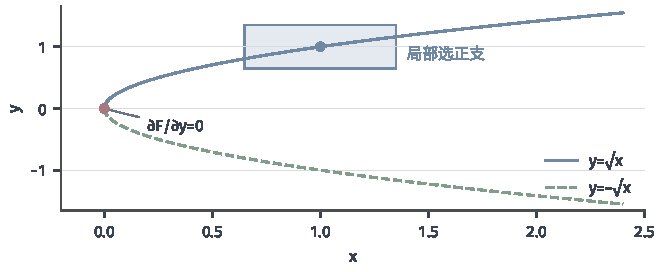
\includegraphics[width=112mm]{figures/01-mathematical-preliminaries-upper/01-mathematical-language-combinatorics-analysis-optimization/matplotlib/comprehension-additions/implicit-branches.pdf}
  \caption{方程$F(x,y)=y^2-x=0$的两支实数解。浅蓝矩形围住$(1,1)$，在该矩形内每个允许的$x$只有正支解，且$F_y=2y\neq0$；红点处$F_y=0$，两支相交。图的两个根都属于同一方程，选定起始解与邻域才确定隐函数分支。}
  \label{fig:vol1-add-implicit-branches}
\end{figure}

\begin{theorem}[隐函数定理]
\label{thm:analysis-implicit-function}
设$F:\mathbb{R}^p\times\mathbb{R}^m\to\mathbb{R}^m$在 $(\bm{a},\bm{b})$的某个开邻域内连续可微， $F(\bm{a},\bm{b})=\bm{0}$，并且关于待解变量的Jacobian矩阵 \[   \bm{D}_{\bm{y}}F(\bm{a},\bm{b})   \in\mathbb{R}^{m\times m} \]
可逆。则存在$\bm{a}$与$\bm{b}$的邻域$U,V$，以及唯一的连续可微函数
$\varphi:U\to V$，使$\varphi(\bm{a})=\bm{b}$，并且对所有
$(\bm{x},\bm{y})\in U\times V$都有
\[
  F(\bm{x},\bm{y})=\bm{0}
  \quad\Longleftrightarrow\quad
  \bm{y}=\varphi(\bm{x}).
\]
其Jacobian矩阵满足
\begin{equation}
  \bm{D}\varphi(\bm{x})
  =
  -
  \bigl[\bm{D}_{\bm{y}}F(\bm{x},\varphi(\bm{x}))\bigr]^{-1}
  \bm{D}_{\bm{x}}F(\bm{x},\varphi(\bm{x})).
\label{eq:analysis-implicit-derivative}
\end{equation}
\end{theorem}

\paragraph{解变化与代回目标后的变化}

定理的存在、局部唯一性和可微性不能由形式求导代替。这里先使用其陈述；第~\ref{sec:analysis-complete-contraction}节建立压缩迭代后，将补全构造证明。一旦确认$\varphi$可微，导数公式也可以直接由链式法则读出：对$F(\bm x,\varphi(\bm x))=\bm0$求导，得到
\[
 \bm D_{\bm x}F+\bm D_{\bm y}F\,\bm D\varphi=\bm0.
\]
左乘关于待解变量的Jacobian的逆，就得到式~\eqref{eq:analysis-implicit-derivative}。这个公式先给出解的移动；若把解代回另一个目标，还需再作一次复合求导。



考虑依赖参数$\theta$的无约束目标$q(z,\theta)$。若局部最优解$z^\star(\theta)$位于定义域内部，它满足驻点方程
\[   F(\theta,z)   =   \frac{\partial q}{\partial z}(z,\theta)   =   0. \]
若$q$二阶连续可微，且 $\partial^2q/\partial z^2$在所考察解处非零，隐函数定理给出该驻点的局部唯一分支。这并不自动说明它是全局最优解；还要由曲率或其他结构核对最优性。
\begin{example}[参数二次目标中的解导数与包络导数]
\label{ex:analysis-parametric-quadratic}
对$\theta>-1$，令
\[   q(z,\theta)   =   \frac12(1+\theta)z^2-\theta z. \]
因为$\theta>-1$，配方得到
\[
  q(z,\theta)=\frac{1+\theta}{2}
  \left(z-\frac{\theta}{1+\theta}\right)^2
  -\frac{\theta^2}{2(1+\theta)}.
\]
平方项的系数为正，所以唯一驻点就是全局最小点。驻点方程为
\[   F(\theta,z)=(1+\theta)z-\theta=0. \]
隐式求导给出
\[   \frac{\mathrm{d}z^\star}{\mathrm{d}\theta}   =   -\frac{\partial F/\partial\theta}{\partial F/\partial z}   =   -\frac{z^\star-1}{1+\theta}. \]
直接消元得到
\[   z^\star(\theta)=\frac{\theta}{1+\theta},   \qquad   \frac{\mathrm{d}z^\star}{\mathrm{d}\theta}   =   \frac{1}{(1+\theta)^2}, \]
两种计算一致。

最优值$V(\theta)=q(z^\star(\theta),\theta)$的链式求导为
\[   V'(\theta)   =   \frac{\partial q}{\partial z}   \frac{\mathrm{d}z^\star}{\mathrm{d}\theta}   +   \frac{\partial q}{\partial\theta}. \]
在内部驻点，第一项因$\partial q/\partial z=0$消失，所以
\begin{equation}
  V'(\theta)
  =
  \left.
  \frac{\partial q}{\partial\theta}
  \right|_{z=z^\star(\theta)}
  =
  \frac12(z^\star)^2-z^\star.
\label{eq:analysis-envelope-quadratic}
\end{equation}
另一方面，直接代回可得
\[   V(\theta)=-\frac{\theta^2}{2(1+\theta)},   \qquad   V'(\theta)   =   -\frac{\theta(\theta+2)}{2(1+\theta)^2}, \]
与式~\eqref{eq:analysis-envelope-quadratic}一致。
\end{example}

式~\eqref{eq:analysis-envelope-quadratic}体现了\term{包络定理}
（envelope theorem）的基本机制：最优值的一阶变化不需要显式乘上最优解导数，因为目标对决策变量的一阶导数在内部最优点为零。但解导数本身并未消失；若关心参数变化后 $z^\star$怎样移动，仍要使用隐式求导。边界解、不可微目标、多重最优解或受约束问题不能直接套用这个简单版本，后续最优化章节会加入相应条件。

\subsection{局部近似的误差控制}

一阶和二阶模型说明近似保留了哪些变化，却没有自动给出可使用的位移范围。下面先沿一段路径控制导数，把局部斜率变成有限变化界；再用Taylor余项把高阶导数与截断误差联系起来，并补全前面驻点分类的充分性论证。

\subsubsection{导数界对有限变化的控制}

\paragraph{中值关系与位移上界}

一点处的线性近似还不能控制一段有限位移。若沿整段路径的变化率都有上界，
中值定理才能把局部信息变成端点之间的误差界。
若$a<b$，$f:[a,b]\to\mathbb{R}$在$[a,b]$上连续、在$(a,b)$上可导，则
\term{中值定理}（mean value theorem）保证存在$c\in(a,b)$使
\begin{equation}
  f(b)-f(a)=f'(c)(b-a).
\label{eq:analysis-mean-value-theorem}
\end{equation}
所以，若区间上$|f'(x)|\leq L$，便有$|f(b)-f(a)|\leq L|b-a|$。这说明有界导数可以推出Lipschitz控制。多元标量函数也可沿线段使用一元中值定理：当连接 $\bm{x}$与$\bm{y}$的线段位于定义域且$f$在线段邻域可微时，
\[   |f(\bm{y})-f(\bm{x})|   \leq   \sup_{0\leq t\leq1}   \lVert\nabla f(\bm{x}+t(\bm{y}-\bm{x}))\rVert_2   \lVert\bm{y}-\bm{x}\rVert_2. \]
这里控制的是标量函数值差。向量的各个输出分量可能在不同位置达到各自的中值斜率，因而未必有一个共同位置能代表整个向量增量。下面直接控制输出增量的范数；积分建立后，也可以沿线段累计Jacobian矩阵。

\paragraph{多方向变化的统一控制}

对向量输出，用线性映射的最大放大倍数替代标量导数的绝对值。
\begin{definition}[欧氏诱导算子范数]
\label{def:analysis-induced-operator-norm}
对矩阵
$\bm{A}\in\mathbb{R}^{s\times r}$，由欧氏范数\term{诱导的算子范数}
（induced operator norm）定义为
\[
  \lVert\bm{A}\rVert_{\mathrm{op}}
  =
  \sup_{\bm{h}\neq\bm{0}}
  \frac{\lVert\bm{A}\bm{h}\rVert_2}{\lVert\bm{h}\rVert_2}
  =
  \sup_{\lVert\bm{h}\rVert_2=1}\lVert\bm{A}\bm{h}\rVert_2.
\]
\end{definition}
它表示线性映射对向量长度的最大放大倍数，定义立即给出
$\lVert\bm{A}\bm{h}\rVert_2
\leq\lVert\bm{A}\rVert_{\mathrm{op}}\lVert\bm{h}\rVert_2$。
例如$\bm A=\operatorname{diag}(2,1)$把第一坐标放大两倍、第二坐标保持不变，
故$\lVert\bm A\rVert_{\mathrm{op}}=2$；最大放大由第一坐标方向达到。
下文$\bm DG$与$\bm J_G$均表示$G$的Jacobian矩阵。
若映射$G$在包含$\bm{y}'$到$\bm{y}$线段的开邻域内连续可微，可以沿线段使用一元中值定理，得到
\begin{equation}
  \begin{aligned}
  \lVert G(\bm{y})-G(\bm{y}')\rVert_2
  &\leq
  \sup_{0\leq t\leq1}
  \left\lVert
    \bm{D}G\bigl(\bm{y}'+t(\bm{y}-\bm{y}')\bigr)
  \right\rVert_{\mathrm{op}}
  \lVert\bm{y}-\bm{y}'\rVert_2.
  \end{aligned}
\label{eq:analysis-operator-mean-value-bound}
\end{equation}
这个向量上界无需预先使用积分公式。若$\bm u=G(\bm y)-G(\bm y')\neq\bm0$，
取单位向量$\bm v=\bm u/\lVert\bm u\rVert_2$，并沿线段定义标量函数
$\phi(t)=\bm v^\top G(\bm y'+t(\bm y-\bm y'))$。
中值定理给出某个$\tau\in(0,1)$，使
\[
 \lVert\bm u\rVert_2
 =\phi(1)-\phi(0)
 =\bm v^\top\bm DG(\bm y'+\tau(\bm y-\bm y'))(\bm y-\bm y').
\]
对右侧使用欧氏内积与算子范数的上界便得到式~\eqref{eq:analysis-operator-mean-value-bound}；
$\bm u=\bm0$时该界直接成立。
因此，任意两点间线段都留在邻域内时，统一的导数范数上界会直接变成Lipschitz常数；若该上界小于$1$，并且$G$把这个邻域映回自身，就得到
第~\ref{sec:analysis-complete-contraction}节将建立的压缩条件。

\subsubsection{高阶近似的截断误差}
\label{sec:analysis-taylor-approximation}

\paragraph{Taylor展开与余项条件}

前面的切线近似只保留一次项，二次修正又加入斜率的变化。若还需要更高精度，可以继续保留同一点处的高阶导数，但必须同时说明截断后遗漏多少。Taylor展开把这些导数组成一个局部多项式，余项则表达原函数与多项式的差。近似阶数与余项界需要一起使用。

对当前的算例，$h=0.1$时一阶近似误差为$0.016$，而二阶近似误差为$0.001$。要判断继续加项是否值得，需要知道误差随$h$和阶数怎样变化，这要求余项的确切表达而不是只比较多项式次数的多少。下面的公式给出余项的一般形式，也说明为什么“阶数越高越准”这一说法必须带上位移尺度与导数上界。

回顾一元Taylor公式：取非负整数$r$，若$f$在连接$x_0$与$x_0+h$的线段的开邻域上
$r+1$阶连续可微，且$h\neq0$，则存在两端之间的$\xi$使
\begin{equation}
  f(x_0+h)=\sum_{k=0}^{r}\frac{f^{(k)}(x_0)}{k!}h^k
  +\frac{f^{(r+1)}(\xi)}{(r+1)!}h^{r+1}.
\label{eq:analysis-taylor-arbitrary-order}
\end{equation}
约定$f^{(0)}=f$，$r$是所保留的最高次数。常数项记录当前函数值，线性项记录斜率，
二次项记录曲率，继续保留高阶项才得到更高阶近似。若沿这条线段
$|f^{(r+1)}|\leq M$，余项的绝对值便不超过$M|h|^{r+1}/(r+1)!$。
所以“高阶近似更准确”还依赖扰动尺度与导数上界，不能只比较多项式的次数。
此处给出的是选取某个中间点的Lagrange余项；若要保留整条线段上各位置的贡献，
第~\ref{sec:analysis-integration-remainders}节将由分部积分建立积分余项，
本节的极值判据并不依赖尚未建立的积分公式。

对前面的$f(x)=x^3-3x$、$x_0=1/2$，三阶展开恰好为
\[
  f(x_0+h)=-\frac{11}{8}-\frac94h+\frac32h^2+h^3.
\]
此处所有四阶及以上导数为零，没有继续舍弃的项。一阶近似$T_1$与二阶近似$T_2$
分别舍弃$\tfrac32h^2+h^3$和$h^3$。图~\ref{fig:analysis-derivative-orders}把两侧扰动放在
同一尺度上比较，显示线性、二次近似怎样接近原曲线，并标出$h=\pm0.1$时的余项。

\begin{figure*}[htbp]
  \centering
  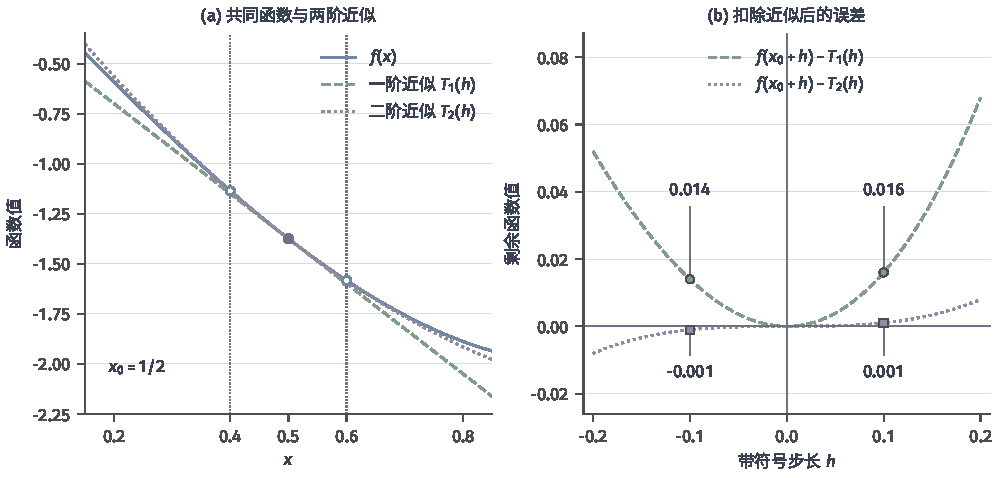
\includegraphics[width=169.0mm]{figures/01-mathematical-preliminaries-upper/01-mathematical-language-combinatorics-analysis-optimization/matplotlib/analysis-derivative-orders/figure.pdf}
  \caption{统一函数 $f(x)=x^3-3x$ 在 $x_0=1/2$ 处的两阶近似，记 $h=x-x_0$。（a）蓝线为真函数，绿虚线为切线近似 $T_1=f(x_0)+f'(x_0)h$，紫点线加入二次项 $f''(x_0)h^2/2$，得到 $T_2$。（b）扣除各近似后的带符号余项分别为 $3h^2/2+h^3$ 与 $h^3$，标出 $h=\pm0.1$ 的精确结果。一阶导数确定切线，二阶导数补充局部曲率；余项的正负表示真值位于近似值的哪一侧。图为解析教学示例。}
  \label{fig:analysis-derivative-orders}
\end{figure*}

\paragraph{多元展开与方向误差}

设连接$\bm{x}$与$\bm{x}+\bm{h}$的线段包含在一个开集内，并且$f$在该开集上二阶连续可微。对一元函数$\phi(t)=f(\bm{x}+t\bm{h})$使用Taylor定理，存在 $\theta\in(0,1)$使
\begin{equation}
  f(\bm{x}+\bm{h})
  =
  f(\bm{x})
  +\nabla f(\bm{x})^{\top}\bm{h}
  +\frac12
  \bm{h}^{\top}
  \nabla^2f(\bm{x}+\theta\bm{h})
  \bm{h}.
\label{eq:analysis-second-order-taylor}
\end{equation}
由Hessian矩阵的连续性，当$\bm{h}\to\bm{0}$时，中间点处的二阶项可以换成基点处的
二阶项，并把差异写成相对于$\lVert\bm h\rVert_2^2$趋零的余项：
\begin{equation}
  f(\bm{x}+\bm{h})
  =
  f(\bm{x})
  +\nabla f(\bm{x})^{\top}\bm{h}
  +\frac12\bm{h}^{\top}\nabla^2f(\bm{x})\bm{h}
  +o(\lVert\bm{h}\rVert_2^2).
\label{eq:analysis-second-order-local-model}
\end{equation}
式~\eqref{eq:analysis-second-order-local-model}是局部结论。若要在一个区域内给出统一余项界，还需控制该区域上的Hessian矩阵连续性或Lipschitz常数，不能仅凭一点处的二阶导数。

前面的Hessian判别需要的正是这种余项控制。下面把已陈述的正定与不定情形补成严格的函数值判断。

正定Hessian矩阵给出更强的充分条件：它要求每个方向都有正曲率，而不只是没有负曲率。
设$f$在$\bm{x}^{\star}$的某个邻域内二阶连续可微，
$\nabla f(\bm{x}^{\star})=\bm{0}$且
$\bm H_\star=\nabla^2f(\bm{x}^{\star})$正定。要把各方向的正曲率变成同一个正下界，
可以在单位球面上考察连续函数$\bm v\mapsto\bm v^\top\bm H_\star\bm v$。
单位球面紧致，故它取到最小值
\[
 \lambda=\min_{\lVert\bm v\rVert_2=1}\bm v^\top\bm H_\star\bm v>0.
\]
正定性保证取到的值仍为正。把任意非零$\bm h$除以其长度，就得到
$\bm h^\top\bm H_\star\bm h\geq\lambda\lVert\bm h\rVert_2^2$。
由Hessian矩阵的连续性，在足够小的球内有
$\lVert\nabla^2f(\bm x)-\bm H_\star\rVert_{\mathrm{op}}\leq\lambda/2$；
算子范数因而把二次型的变化量控制在$(\lambda/2)\lVert\bm h\rVert_2^2$以内，
邻近位置的曲率下界仍至少为$(\lambda/2)\lVert\bm h\rVert_2^2$。
用式~\eqref{eq:analysis-second-order-taylor}
的中间点表达式，即可把这个曲率下界变成函数值下界；具体地，充分靠近时有
\[   f(\bm{x}^{\star}+\bm{h})-f(\bm{x}^{\star})   \geq   \frac{\lambda}{4}\lVert\bm{h}\rVert_2^2>0 \]
对充分小的非零$\bm{h}$成立，故$\bm{x}^{\star}$是严格局部极小点。负定情形给出严格局部极大点。

若驻点处Hessian矩阵不定，分别选取二次型为正和为负的方向。
沿每个固定方向把扰动写成$t\bm v$时，余项为$o(t^2)$，因此充分小的非零$t$不会改变
非零二次项的符号，函数值因而分别增加和减小，该点称为\term{鞍点}（saddle point）。
例如$f(x,y)=x^2-y^2$的原点就是鞍点。
若Hessian矩阵仅半正定或半负定，且在某些非零方向上二次型为零，二阶判据可能没有结论，
必须查看更高阶项或函数的其他结构。上述必要条件还假定点位于无约束开集内部；
边界极小点的梯度可以不为零，受约束问题需要后续章节的可行方向与乘子条件。

\section{函数的积分与整体累计}
\label{sec:analysis-classical-integration}

微分描述一点附近怎样变化，积分研究一个范围内的数值怎样累计。困难是有限分割得到的和依赖分割与取样位置，必须证明细分后这些差别消失。下面先建立积分及其存在范围，再研究原函数、分步计算和坐标变换，最后沿路径和区域累计导数，说明端点与边界项来自哪里。这里采用有界区间与规则区域上的经典版本。

\subsection{积分的存在与累计范围}

从连续函数的面积累计开始，有限分割给出一组可核对的近似。上下和将所有取样选择夹在共同范围内，可积性要求这个范围能缩到任意小。建立有界区间上的积分后，再把无界函数和无穷区间作为截断极限处理。

\subsubsection{有界函数的分割累计}
\label{sec:analysis-riemann-integral}

\paragraph{黎曼和、上下和与分割细化}

要累计$f:[a,b]\to\mathbb R$在区间上的贡献，先选分割$P:a=x_0<x_1<\cdots<x_n=b$。在第$i$个小区间选取$\xi_i\in[x_{i-1},x_i]$，用矩形贡献$f(\xi_i)(x_i-x_{i-1})$代替这一段累计，得到\term{黎曼和}（Riemann sum）
\[
 S(f,P,\bm\xi)=\sum_{i=1}^n f(\xi_i)(x_i-x_{i-1}).
\]
暂时假定$f$有界，令$m_i=\inf_{[x_{i-1},x_i]}f$、$M_i=\sup_{[x_{i-1},x_i]}f$，便得到所有取样都满足的共同下界和上界：
\begin{equation}
 L(f,P)=\sum_i m_i(x_i-x_{i-1})
 \ \leq\ S(f,P,\bm\xi)\ \leq\
 U(f,P)=\sum_i M_i(x_i-x_{i-1}).
\label{eq:analysis-riemann-upper-lower-sums}
\end{equation}
增加分割点会提高下和或使它不变，降低上和或使它不变。不同分割可以取共同细化，因此任一下和不超过任一上和。若下和所能达到的上确界与上和所能达到的下确界相等，所有分割累计就确定同一个值。
\begin{definition}[黎曼可积与黎曼积分]
\label{def:analysis-riemann-integral}
设$a<b$且$f:[a,b]\to\mathbb R$有界。若
\[
 \sup_P L(f,P)=\inf_P U(f,P),
\]
则称$f$在$[a,b]$上\term{黎曼可积}（Riemann integrable），共同值称为\term{黎曼积分}（Riemann integral），记为$\int_a^b f(x)\,\mathrm dx$。
\end{definition}
等价的误差判据是：对每个$\varepsilon>0$都存在分割$P$使$U(f,P)-L(f,P)<\varepsilon$。共同值存在时，分别选出距它小于$\varepsilon/2$的下和与上和，再取共同细化即可证明这一方向；反过来，任一分割上的上下和差都控制两确界之差，所以任意小的差迫使它们相等。这也等价于分割的最大小区间长度趋零时，所有取样黎曼和趋向同一值；下面的存在性证明直接使用上下和判据。

若$f,g$均可积，细分同时控制两者在每个小区间的振荡，便可控制$f+g$的振荡。由有限和的线性并取极限，得到积分的线性。若$f\leq g$，每个黎曼和都保持次序，积分也保持次序。因此$|f-g|\leq M$时有$|\int_a^b f-\int_a^b g|\leq M(b-a)$。绝对值运算不扩大每段振荡，因此可积的$f$也有可积的$|f|$，且$|\int f|\leq\int|f|$。把一个区间分成相邻两段时，分割和相加，取极限也得到积分的区间可加性。这些性质把函数误差转成累计误差，后面会反复使用。

\paragraph{连续、有限跳变与不可积的对照}

若$f$在$[a,b]$上连续，紧致性先保证它有界且一致连续。给定$\varepsilon>0$，选$\delta>0$使两点相距小于$\delta$时函数值相差小于$\varepsilon/(b-a)$。当分割各段长度都小于$\delta$，每段的$M_i-m_i$不超过这一阈值，故
\[
 U(f,P)-L(f,P)=\sum_i(M_i-m_i)(x_i-x_{i-1})\leq\varepsilon.
\]
所以紧区间上的连续函数黎曼可积。这里一致连续负责同时控制全部小区间，只有逐点连续的定义尚不能直接选出共同分割尺度。

连续性是充分条件，不是必要条件。若有界函数只有有限个跳变，可以先用总长度任意小的短区间包住这些位置；它们对上下和差的贡献不超过函数振幅乘总长度。其余有限个闭区间上连续，再用一致连续控制。于是有限跳变仍可积，在有限个位置改值也不改变积分。

相反，令$d(x)=\mathbb I\{x\in\mathbb Q\}$，定义在$[0,1]$。每个非退化小区间都有有理数和无理数，因此每段$m_i=0$、$M_i=1$，任意分割都给出$L(d,P)=0$、$U(d,P)=1$。这个函数有界，却无法使上下累计接近，所以不黎曼可积。问题在于每一小段都保留最大振荡，而不是函数值很大。

\subsubsection{无界函数与无穷范围的累计}
\label{sec:analysis-improper-integrals}

\paragraph{反常积分的截断极限}

黎曼积分要求函数在有限闭区间上有界。若奇异性只发生在端点，可以先避开它再取极限。例如$f$在每个$[c,b]$（$a<c<b$）上黎曼可积，定义
\[
 \int_a^b f(x)\,\mathrm dx:=\lim_{c\downarrow a}\int_c^b f(x)\,\mathrm dx,
\]
前提是右侧存在有限极限。无穷区间则令$\int_a^\infty f=\lim_{R\to\infty}\int_a^R f$。这些通过截断建立的积分称为\term{反常积分}（improper integral）。有多个奇异端点或两端无穷时，应分别检查每一端，不能只用相互抵消的对称截断代替。

以正函数$x^{-p}$说明位置的重要性。对$p>0$，在$[2^k,2^{k+1}]$上的累计满足
\[
 2^{-p}2^{k(1-p)}\leq\int_{2^k}^{2^{k+1}}x^{-p}\,\mathrm dx\leq2^{k(1-p)}.
\]
这是把函数在该段的最小值和最大值分别乘区间长度。$p>1$时上界随$k$几何衰减，有限几何和有共同上界，所以尾部积分收敛；$0<p\leq1$时各段至少贡献一个不趋零的正量，累计发散。$p\leq0$时$x^{-p}\geq1$于$x\geq1$，也发散。

同样比较靠近$0$的各段$[2^{-(k+1)},2^{-k}]$，在$p>0$时累计介于$2^{k(p-1)}/2$与$2^{p-1}2^{k(p-1)}$之间，故局部累计恰在$p<1$时有限；$p\leq0$时函数还能连续延拓到$0$，本来就可积。于是$\int_0^1x^{-p}\,\mathrm dx$恰在$p<1$时有限，$\int_1^\infty x^{-p}\,\mathrm dx$恰在$p>1$时有限。这里仅用分段常数比较与有限几何和，不提前使用下一小节的原函数计算。

\paragraph{收敛、绝对收敛与尾部误差}

若$\int |f|$对应的反常积分有限，有限区间上的$|\int f|\leq\int|f|$就能统一控制任意两次截断的差。实数完备性保证$\int f$收敛，这称为绝对收敛。对非负函数，比较$f\leq g$且$\int g<\infty$即可得到收敛与尾部界。例如$p>1$时，按$[2^jR,2^{j+1}R]$分段比较得到
\[
 \int_R^{2^{K+1}R} x^{-p}\,\mathrm dx
 \leq R^{1-p}\sum_{j=0}^K 2^{j(1-p)}
 \leq\frac{R^{1-p}}{1-2^{1-p}},
\]
右侧与$K$无关，也就控制了整个无穷尾部；它随$R$增大而趋零，给出截断到$R$之后的误差。

正负抵消也可能产生有限极限。令$f(x)=(-1)^{k+1}/k$于$k\leq x<k+1$，其中$k=1,2,\ldots$。每个有限截断只含有限个跳变，整数端点的积分为$s_N=1-1/2+\cdots+(-1)^{N+1}/N$。偶数项$s_{2N}$递增且不超过$1$，所以有有限极限；相邻奇数项与其差为$1/(2N+1)\to0$，二者趋于同一值。非整数截断与相邻整数截断的积分差不超过$1/N$，因此$\int_1^\infty f$收敛。

但$\int_1^{N+1}|f|=\sum_{k=1}^N1/k$无界：从$k=2^j$到$2^{j+1}-1$的一组至少贡献$1/2$。所以这一反常积分收敛却不绝对收敛，正负贡献的抵消不可省略。后章的勒贝格可积要求绝对值累计有限，不能把这类条件收敛直接沿用为同一个可积判断。

\subsection{积分的计算与坐标变换}

积分定义解决了累计是否存在，但直接计算分割极限通常繁琐。先用原函数把区间累计变成端点差，再把多变量累计拆成分步计算，最后在更合适的坐标中改写函数与体积。每次变化都必须同时保留累计范围、方向和权重。

\subsubsection{区间积分的原函数计算}
\label{sec:analysis-integration-remainders}

\paragraph{累计函数与微积分基本定理}

先回顾微积分基本定理的连续版本。若$g$在$[a,b]$上连续，
$H(x)=\int_a^xg(t)\,\mathrm dt$在内点处满足$H'(x)=g(x)$；
若$H\in C^1([a,b])$，则$\int_a^bH'(x)\,\mathrm dx=H(b)-H(a)$。
这里$C^1$表示一阶连续可微，在闭区间端点采用单侧导数的连续延拓。
第一条可由
$[H(x+h)-H(x)]/h-g(x)=h^{-1}\int_x^{x+h}(g(t)-g(x))\,\mathrm dt$
和连续性得到；第二条再对$H(x)-H(a)-\int_a^xH'(t)\,\mathrm dt$
使用零导数蕴含常值的中值定理。这说明所用的是连续导数的积分，更一般的导数恢复条件将在第~\ref{chap:measurable-functions}章研究。

\paragraph{分部积分与积分余项}

有些乘积的积分难算，但把导数转移到另一个因子后会简化。分部积分就是这种转移规则，代价是增加边界贡献。若$u,v\in C^1([a,b])$，由乘积求导$(uv)'=u'v+uv'$并在$[a,b]$上积分，可得
\begin{equation}
  \int_a^b u(x)v'(x)\,\mathrm{d}x
  =
  [u(x)v(x)]_a^b
  -
  \int_a^b u'(x)v(x)\,\mathrm{d}x.
\label{eq:analysis-integration-by-parts}
\end{equation}
例如，取$u(x)=x$、$v'(x)=e^x$，得到 $\int_0^1xe^x\,\mathrm{d}x=[xe^x]_0^1-\int_0^1e^x\,\mathrm{d}x=1$。边界项不能无故删除；只有在函数于边界消失、区域无边界，或衰减速度足以使无穷远边界项趋零时才能省略。

分部积分还能把第~\ref{sec:analysis-taylor-approximation}节的局部二阶变化累计成有限位移的
余项。设连接$\bm{x}$与$\bm{x}+\bm{h}$的线段包含在一个开集内，且$f$在该开集上二阶
连续可微。令$\phi(t)=f(\bm{x}+t\bm{h})$，对$(1-t)\phi''(t)$在$[0,1]$上分部积分，得到
\[
  \int_0^1(1-t)\phi''(t)\,\mathrm{d}t
  =-\phi'(0)+\phi(1)-\phi(0).
\]
用链式法则代回，便得到不挑选中间点的Taylor积分余项：
\[   f(\bm{x}+\bm{h})   =   f(\bm{x})   +\nabla f(\bm{x})^{\top}\bm{h}   +   \int_0^1(1-t)   \bm{h}^{\top}\nabla^2f(\bm{x}+t\bm{h})\bm{h}\,\mathrm{d}t. \]
权重$1-t$说明越靠近位移起点的曲率贡献被累计得越多；该表达式与前面的中间点余项
描述同一有限变化，但保留了整条线段上的曲率信息。

一般阶数也由同一操作得到。设$f$在连接$x_0$和$x_0+h$的线段邻域内
$r+1$阶连续可微，$r\geq0$，令$\phi(t)=f(x_0+th)$。
记
\[
 I_r=\frac1{r!}\int_0^1(1-t)^r\phi^{(r+1)}(t)\,\mathrm dt.
\]
基本定理给出$I_0=\phi(1)-\phi(0)$；对$r\geq1$分部积分，
\[
 I_r=-\frac{\phi^{(r)}(0)}{r!}
       +\frac1{(r-1)!}\int_0^1(1-t)^{r-1}\phi^{(r)}(t)\,\mathrm dt
     =-\frac{\phi^{(r)}(0)}{r!}+I_{r-1}.
\]
逐次代入并用$\phi^{(k)}(0)=h^k f^{(k)}(x_0)$，便得
\begin{equation}
 f(x_0+h)=\sum_{k=0}^r\frac{f^{(k)}(x_0)}{k!}h^k
 +\frac{h^{r+1}}{r!}
   \int_0^1(1-t)^r f^{(r+1)}(x_0+th)\,\mathrm dt.
\label{eq:analysis-taylor-integral-remainder}
\end{equation}
参数化$x_0+th$同时处理正、负$h$。若$|f^{(r+1)}|\leq M$，积分权重的总量为
$1/(r+1)$，故余项不超过$M|h|^{r+1}/(r+1)!$，与前面的中间点余项界一致。
例如立方函数在$r=2$时有$f'''=6$，余项就是
$(h^3/2)\int_0^1 6(1-t)^2\,\mathrm dt=h^3$。
多元函数沿$\phi(t)=f(\bm x+t\bm h)$使用同一公式；$r=1$便还原前述Hessian积分余项。

\subsubsection{多变量积分的分步计算}

\paragraph{区域分割与体积累计}

在矩形$R=[a,b]\times[c,d]$上，分别划分两个坐标，把每个小矩形的面积乘以其中一个函数值后求和。若$f$在$R$上连续，紧致性给出统一振荡控制，所以分割细化时得到与取样无关的二重积分。更高维用小长方体体积作同样构造。

非矩形的有界区域$D$可以放入一个大矩形，把区域外的贡献设为零。这里采用规则区域：边界能用有限个光滑片段或曲面片描述，边界附近能够被总面积或总体积任意小的小块覆盖。这一条件保证边界小块对有界函数的上下和差贡献趋零。它是经典区域积分的条件，不要求事先建立一般集合的测度。

\paragraph{积分次序与区域描述}

矩形上的连续函数可以先按一个坐标累计，再按另一个坐标累计：
\[
 \int_R f(x,y)\,\mathrm d(x,y)
 =\int_a^b\left(\int_c^d f(x,y)\,\mathrm dy\right)\mathrm dx
 =\int_c^d\left(\int_a^b f(x,y)\,\mathrm dx\right)\mathrm dy.
\]
有限双重和本来就能交换相加次序；连续性提供共同的分割误差界，允许把这一关系传到积分极限。若区域写为$a\leq x\leq b$、$\alpha(x)\leq y\leq\beta(x)$，其中上下边界连续，内积分上下限就应使用$\alpha(x),\beta(x)$。改变积分次序时应重新描述同一个区域。

例如$D=\{(x,y):0\leq y\leq x\leq1\}$上累计$1$，先对$y$积分得到$\int_0^1\int_0^x1\,\mathrm dy\,\mathrm dx=1/2$；反过来，同一区域为$0\leq y\leq1$、$y\leq x\leq1$，故$\int_0^1\int_y^11\,\mathrm dx\,\mathrm dy=1/2$。若只交换微分符号而保留原来的限，就已经改变区域。一般可测函数或存在奇异抵消的情形，需要下一章的分步积分定理单独核验。

\subsubsection{坐标变化后的积分计算}
\label{sec:analysis-coordinate-change-integral-applications}

\paragraph{一元换元与链式法则}

设$g$在包含$T([a,b])$的区间上连续，$T\in C^1([a,b])$。取$g$的原函数$G$，链式法则给出$(G\circ T)'(x)=g(T(x))T'(x)$。再用基本定理得到
\[
 \int_a^b g(T(x))T'(x)\,\mathrm dx
 =G(T(b))-G(T(a))=\int_{T(a)}^{T(b)}g(u)\,\mathrm du.
\]
这里$\int_v^u=-\int_u^v$保留有向端点。若把换元理解为一一对应地累计普通长度，则还需在当前区间保证$T$单调，并用$|T'|$补偿方向翻转。

\paragraph{Jacobian与体积权重}

多元换元同时改变函数表达和小区域体积。设$D$是有界规则区域，$\overline D$包含在开集$U\subseteq\mathbb R^d$内；$T:U\to V$为一一对应的连续可微映射，其逆也连续可微，且$\det\bm J_T\neq0$。若$g$在$T(\overline D)$上连续，则经典换元公式为
\begin{equation}
 \int_{T(D)}g(\bm y)\,\mathrm d\bm y
 =\int_D g(T(\bm x))\left|\det\bm J_T(\bm x)\right|\,\mathrm d\bm x.
\label{eq:analysis-multivariate-change-variables}
\end{equation}
Jacobian描述局部线性变化，行列式的绝对值是普通体积的缩放比例。绝对值使坐标方向翻转后体积仍为正。公式可以从小块上的线性近似及统一误差控制证明；逐点线性化只说明局部缩放，严格的整体公式还要控制分割后的误差与像集重叠。这里陈述这一经典版本，后章再扩大到非负可测或绝对可积函数。

\begin{example}[极坐标中的面积权重]
\label{ex:analysis-polar-coordinate-jacobian}
令$D=\{\bm{x}\in\mathbb{R}^2:\lVert\bm{x}\rVert_2\leq1\}$，并令
$T(r,\theta)=(r\cos\theta,r\sin\theta)$。在开集
$(0,1)\times(0,2\pi)$上，$T$是到开圆盘内部去掉原点和正$x$轴径向接缝后的区域的
连续可微双射，逆映射也连续可微。其Jacobian矩阵的行列式为
\[   \det
\begin{bmatrix}     \cos\theta & -r\sin\theta\\     \sin\theta & r\cos\theta
\end{bmatrix}   =r. \]
为了避开原点和接缝，可先限制$\varepsilon\leq r\leq1-\varepsilon$、$\varepsilon\leq\theta\leq2\pi-\varepsilon$，在每个这样的闭矩形上使用经典换元。遗漏的中心小圆盘、外侧窄环与接缝窄扇形面积随$\varepsilon\downarrow0$趋零；对有界被积函数，它们的累计贡献也趋零。因此取极限得到
\[   \int_D1\,\mathrm{d}\bm{x}   =   \int_0^{2\pi}\int_0^1r\,\mathrm{d}r\,\mathrm{d}\theta   =\pi. \]
这里积分上下限包含端点不改变积分值。若参数化在一片有正面积或体积的区域上重复覆盖，则不能直接使用
上述双射版本，否则同一点会被重复计数。
\end{example}

图~\ref{fig:vol1-add-polar-area-weight}说明半径因子来自哪里。同样的角度变化在较大半径处扫过更长的弧，故同样大小的参数块对应更大的面积，积分权重必须随半径变化。
\begin{figure}[!htb]
  \centering
  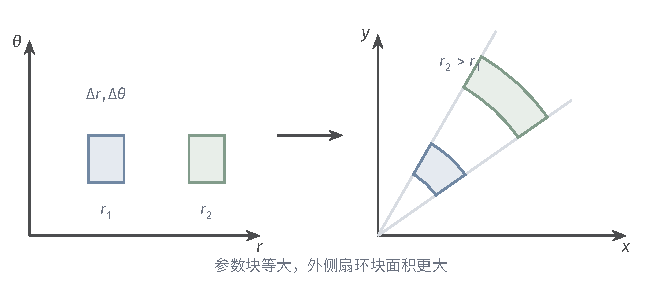
\includegraphics[width=112mm]{figures/01-mathematical-preliminaries-upper/01-mathematical-language-combinatorics-analysis-optimization/tikz/comprehension-additions/polar-area-weight.pdf}
  \caption{极坐标映射中的两个等大参数块，具有相同的$\Delta r,\Delta\theta$，但外侧半径$r_2$较大。对应扇环块的精确面积为$(r\Delta r+(\Delta r)^2/2)\Delta\theta$，一阶项为$r\Delta r\Delta\theta$，因此面积元为$r\,\mathrm dr\,\mathrm d\theta$。图只比较局部块，坐标原点与接缝的处理见正文。}
  \label{fig:vol1-add-polar-area-weight}
\end{figure}

\subsection{路径与区域中的边界关系}

前面在区域中累计函数值，现在改为累计导数。沿路径累计梯度留下端点差，在区域内累计散度留下边界净通量。两者都能由小段或小区域内部贡献相消理解，但方向、权重和光滑性条件不同，下面分别建立。

\subsubsection{路径累计与端点变化}

\paragraph{弧长累计与有向线积分}

换元仍是在同维区域内计算体积积分；如果贡献只沿一条路径累积，就应改用弧长或带方向的路径增量，不能继续套用全空间体积权重。设分段连续可微路径$\gamma:[a,b]\to\mathbb{R}^d$。对沿路径连续的标量函数
$h:\mathbb{R}^d\to\mathbb{R}$，标量线积分定义为
\[
  \int_\gamma h\,\mathrm{d}s
  =
  \int_a^b h(\gamma(t))\lVert\gamma'(t)\rVert_2\,\mathrm{d}t.
\]
速度的范数把参数增量换成弧长，因此反转路径方向不改变该积分。对沿路径连续的向量场
$\bm{F}:\mathbb{R}^d\to\mathbb{R}^d$，向量场线积分则定义为
\[   \int_{\gamma}\bm{F}\mathbin{\cdot}\mathrm{d}\bm{r}   =   \int_a^b   \bm{F}(\gamma(t))^{\top}\gamma'(t)\,\mathrm{d}t. \]

速度范数换算普通弧长，带方向的速度向量则保留行进方向。路径反向时，前者不变，后者变号；因此二者累计的是不同对象。

\paragraph{梯度场的端点差}

若$\bm{F}=\nabla\phi$且$\phi$连续可微，链式法则给出
\begin{equation}
  \int_{\gamma}\nabla\phi\mathbin{\cdot}\mathrm{d}\bm{r}
  =
  \phi(\gamma(b))-\phi(\gamma(a)).
\label{eq:analysis-line-integral-gradient}
\end{equation}
因此梯度场的路径积分只依赖端点。向量场线积分在路径方向反转时变号；若漏掉参数化导数
$\gamma'(t)$，就会丢失方向和行进速度的信息。

\begin{example}[同一路径上的长度、端点差与环流]
\label{ex:analysis-path-integral-comparison}
取单位圆的上半圆路径$\gamma(t)=(\cos t,\sin t)$，$0\leq t\leq\pi$。
它的速度范数恒为$1$，所以$\int_\gamma1\,\mathrm ds=\pi$。
取$\phi(x,y)=x$，则$\nabla\phi=(1,0)^\top$，
\[
 \int_\gamma\nabla\phi\mathbin{\cdot}\mathrm d\bm r
 =\int_0^\pi-\sin t\,\mathrm dt=-2
 =\phi(-1,0)-\phi(1,0).
\]
换成旋转场$\bm F(x,y)=(-y,x)^\top$时，
$\bm F(\gamma(t))^\top\gamma'(t)=1$，沿上半圆的积分为$\pi$。
但沿同样端点的直径路径$\eta(t)=(1-2t,0)$，$0\leq t\leq1$，
内积恒为零，积分为$0$。向量场连续甚至光滑，也不能单独保证路径无关。
沿完整单位圆逆时针一周，这个旋转场的积分为$2\pi$；梯度场沿闭合路径的端点差
必须为零，所以它不可能在整个平面上写成一个连续可微势函数的梯度。
\end{example}

\subsubsection{区域累计与边界通量}

\paragraph{散度与内部贡献相消}

路径积分沿行进方向累计，通量则计算穿过边界的贡献。在向量场
$\bm F=(F_1,\ldots,F_d)^\top$中，散度定义为
$\nabla\mathbin{\cdot}\bm F=\sum_{i=1}^d\partial F_i/\partial x_i$；
它把各坐标方向的局部流出率相加。相邻小区域的公共边界法向相反，
内部交换在总和中相消，剩下的应是外边界的净流出。


对一个小长方体，每个坐标方向上两面的净流出约等于该方向的偏导数乘体积。把小块相加，内部公共面的法向相反，所以贡献抵消；只有外边界保留下来。

\paragraph{散度定理与多元分部积分}

以下采用经典的规则区域版本：$\Omega$是有界开区域，其边界由有限个$C^1$
曲面片组成，每个光滑片附近区域位于边界的一侧，片间接缝可以被总边界面积任意小的细片覆盖。
光滑区域、多边形和通常的多面体均符合这一条件。若向量场$\bm{F}$
在$\overline{\Omega}$的一个开邻域内连续可微，
\term{散度定理}（divergence theorem）写成
\begin{equation}
  \int_{\Omega}\nabla\mathbin{\cdot}\bm{F}\,\mathrm{d}\bm{x}
  =
  \int_{\partial\Omega}\bm{F}^{\top}\bm{n}\,\mathrm{d}S,
\label{eq:analysis-divergence-theorem}
\end{equation}
其中$\bm{n}$是外单位法向量，$\mathrm dS$表示边界上的面积元素。这个公式把区域内部与区域边界两种积分联系起来；左边汇总区域内部的局部流出率，右边计算穿过边界的净通量。普通多边形角点和多面体接缝已包含在上述分片条件内。对于不满足上述分片及局部单侧条件的边界，或涉及无界区域、弱导数的情形，需要另用相应版本并重新核对边界项。分部积分、路径积分与散度定理共同说明，局部导数进入整体积分时， 通常会留下不可忽略的边界信息。

例如单位开圆盘$\Omega$上的$\bm F(x,y)=(x,y)^\top$有散度$2$，
故左边为$2\pi$。边界参数化$\gamma(t)=(\cos t,\sin t)$，$0\leq t\leq2\pi$，
外单位法向就是$\bm n=\gamma(t)$，弧长元素为$\mathrm dS=\mathrm dt$；
因此$\bm F^\top\bm n=1$，右边也为$2\pi$。
改用内法向会得到$-2\pi$，这不是同一定理中的方向约定。
前例的旋转场散度为零，且在圆周上始终与法向垂直，所以通量为零，
尽管沿切向的环流为$2\pi$。这一区别说明线积分和通量计算的不是同一种贡献。

取连续可微标量函数$u,v$，令$\bm F=u\nabla v$，并假定$v$二阶连续可微。乘积法则给出$\nabla\mathbin\cdot(u\nabla v)=\nabla u^\top\nabla v+u\Delta v$，其中$\Delta v=\sum_i\partial^2v/\partial x_i^2$称为Laplace算子。代入散度定理得
\[
 \int_\Omega u\Delta v\,\mathrm d\bm x
 =\int_{\partial\Omega}u\nabla v^\top\bm n\,\mathrm dS
  -\int_\Omega\nabla u^\top\nabla v\,\mathrm d\bm x.
\]
这个多元分部积分公式将二阶导数转给另一个因子，同时保留法向边界项；边界条件是否使该项为零，需要在具体问题中判断。

\section{函数逼近与运算的极限}
\label{sec:analysis-function-convergence-essential-bounds}

现在让被研究的函数本身随索引变化。固定一个输入后仍是一列数，但各位置的趋近速度可以不同，积分还会累计误差发生的范围。下面先规定函数列的共同误差尺度，再分别检查连续性、积分和求导是否保留，最后研究部分和与更新规则生成的特殊逼近。经典方法失效的反例将明确引出下一章的任务。

\subsection{函数列的误差尺度与极限存在}

逐点误差只检查一个位置，一致误差要求同一轮近似控制全部位置。先用幂函数列分清这两个量词次序，再用一致柯西条件判断未知函数极限的存在。这里不要求输入已经有距离，也不要求各函数连续或可积。

\subsubsection{逐点误差与统一误差}

\paragraph{各位置分别趋近}

固定一个输入以后，比较的只是一列实数。这里不需要函数可微或可积，甚至不需要
在输入集合上指定距离；函数值仍按实数绝对值比较。
\begin{definition}[逐点收敛]
\label{def:analysis-pointwise-almost-everywhere-convergence}
设$f_n,f:X\to\mathbb{R}$。若
\[
 \begin{gathered}
  \forall x\in X,\quad
  \forall\varepsilon>0,\quad
  \exists N=N(x,\varepsilon)\in\mathbb N,\\
  \forall n\geq N,\quad
  |f_n(x)-f(x)|<\varepsilon,
 \end{gathered}
\]
即对每个$x$都有$\lim_n f_n(x)=f(x)$，称$f_n$逐点收敛到$f$。
\end{definition}


例如$f_n(x)=x^n$在$[0,1]$上，对每个$x<1$趋于$0$，在$x=1$却始终等于$1$。所以逐点极限为$f(x)=0$（$x<1$）、$f(1)=1$；这一写法先固定位置，再让$n$增加。

\paragraph{整个范围的共同控制}

即使每个输入处的误差最终都很小，开始稳定的时刻仍可能依赖输入。
若希望一次选定迭代次数后就控制全部输入，需要更强的一致条件。

这个区别不是纯粹的技术细节。实际使用近似函数时，通常要先决定计算到第几轮，
再把这个近似函数交给下一步使用；而逐点收敛只保证每个位置最终会变准，不保证在
固定的轮数上处处都准。一致收敛正是允许“先定轮数、再要求处处达标”的条件。
\begin{definition}[函数列的一致收敛]
\label{def:analysis-uniform-convergence}
设$X$为非空集合，$f_n,f:X\to\mathbb R$。若
\[
  \forall\varepsilon>0,\quad
  \exists N=N(\varepsilon)\in\mathbb N,\quad
  \forall x\in X,\quad
  \forall n\geq N,\quad
  |f_n(x)-f(x)|<\varepsilon,
\]
就称$f_n$在$X$上一致收敛到$f$。等价地，
\begin{equation}
  \lVert f_n-f\rVert_{\infty}
  :=
  \sup_{x\in X}|f_n(x)-f(x)|
  \longrightarrow0.
\label{eq:analysis-uniform-convergence}
\end{equation}
这里的上确界检查全部输入，不排除任何位置。
\end{definition}


两条定义的区别落在量词次序。逐点收敛允许$N$依赖$x$；一致收敛把$\exists N$
移到$\forall x$之前，同一个$N$必须同时控制全部输入。区别不在“趋近”这个词，
而在误差阈值之后允许谁依赖谁。下面用同一列函数比较这两种控制。

在$[0,1]$上取$f_n(x)=x^n$。它逐点收敛到
\[
 f(x)=
 \begin{cases}
  0,&0\leq x<1,\\
  1,&x=1.
 \end{cases}
\]
每个固定的$0<x<1$都有$x^n\to0$，端点$1$处的函数值与极限值则始终都为$1$，误差为零。
但对每个$n$，$\sup_{x\in[0,1]}|f_n(x)-f(x)|=\sup_{0\leq x<1}x^n=1$，所以收敛不一致。
从量词看，固定$\varepsilon=1/2$后，无论选多大的$N$，在$n=N$时
总能选$x_N=(3/4)^{1/N}<1$，使误差$x_N^N=3/4>\varepsilon$。
失败的位置可以随$n$移动；不能把“每个位置最终变小”改写成“某一轮以后所有位置都小”。
若把范围缩为$[0,a]$，其中$0\leq a<1$，则上确界误差为$a^n\to0$，同一公式又变成一致收敛。

\subsubsection{未知极限函数时的收敛判断}

\paragraph{一致柯西条件}

前面都先给出候选极限，再判断误差；实际构造时可能只知道后面的函数彼此很近。
令$S$为任意非空集合，$\mathcal F_{\mathrm b}(S)$为所有有界实函数$S\to\mathbb{R}$的集合，配备普通上确界范数
\[   \lVert f\rVert_{\infty}   =   \sup_{x\in S}|f(x)|. \]
这里的元素是整个函数，距离比较它们在全部输入上的最大误差。
所比较的是两个函数之间的距离$\lVert f-g\rVert_\infty$，它检查每个输入而不排除例外位置。
一致柯西条件就是
\[
 \forall\varepsilon>0,\quad\exists N,\quad
 \forall m,n\geq N,\quad\forall x\in S,\quad
 |f_m(x)-f_n(x)|<\varepsilon.
\]

\paragraph{一致极限的存在与归属}

这个空间完备。事实上，若$(f_n)$满足上述条件，对每个固定$x$，
$(f_n(x))$是实柯西列，故存在$f(x)=\lim_n f_n(x)$。
取一个$n_0$使$\lVert f_n-f_{n_0}\rVert_\infty\leq1$对所有充分大的$n$成立，
再令$n\to\infty$，得到$|f(x)|\leq|f_{n_0}(x)|+1$，所以$f$有界。
对任意$\varepsilon>0$，选$N$使$m,n\geq N$时
$\lVert f_m-f_n\rVert_\infty<\varepsilon/2$。固定$n\geq N$并令$m\to\infty$，
对所有$x$都有$|f(x)-f_n(x)|\leq\varepsilon/2$，于是
$\lVert f-f_n\rVert_\infty\leq\varepsilon/2<\varepsilon$。
这证明$f_n$在该空间中收敛到$f$，而不只是分别得到了各个点的极限。

\subsection{极限下的性质与运算保持}

误差尺度确定后，还需分别检查希望保留的对象。连续性只用函数值的三角误差分解，积分会累计整个范围，求导还会把相邻位置的差除以很小的位移。因此三个保持问题需要各自证明，不能由其中一个自动推出另两个。

\subsubsection{连续性是否保留}

\paragraph{一致极限的连续性}

前面的完备性说明一致柯西列有函数极限，还可以追问原函数的性质是否保留。
若度量空间$X$上的实函数$f_n$连续，且$f_n$一致收敛到$f$，则$f$连续。
固定$x\in X$与$\varepsilon>0$，先选$n$使$\lVert f-f_n\rVert_\infty<\varepsilon/3$，
再由这个$f_n$在$x$处连续，选$\delta>0$控制
$|f_n(x')-f_n(x)|<\varepsilon/3$。于是$d(x,x')<\delta$时，
\[
 |f(x')-f(x)|
 \leq |f(x')-f_n(x')|+|f_n(x')-f_n(x)|+|f_n(x)-f(x)|
 <\varepsilon.
\]
一致误差同时控制两端，连续性才被保留。仅逐点收敛没有这个共同控制；上面的$x^n$
例子中，各项连续，极限在$x=1$处却不连续。这里回用的是第~\ref{sec:analysis-continuous-limits}节的连续性，并未使用积分。

\paragraph{逐点极限中的跳变}

一致收敛是这个结论的充分条件，不是极限连续的必要条件。
例如$x^n$在$[0,1)$上的逐点极限恒为零，仍然连续，但其上确界误差始终为$1$。
这不反驳上面的定理，只说明有些不满足统一误差条件的函数列也恰好保留了连续性。

同一幂函数列在闭区间上的极限于$1$处不连续。每个固定位置最终准确仍然不够，因为靠近$1$的困难位置随$n$不断移动，找不到共同轮数来完成连续性证明中的两端误差控制。

\subsubsection{积分是否可以交换极限}
\label{sec:analysis-classical-limit-integral}

\paragraph{有限区间上的一致误差界}

设$f_n$在固定区间$[a,b]$上黎曼可积，并一致收敛到$f$。先说明极限仍可积：固定一个使$\lVert f-f_n\rVert_\infty<\eta$的$n$，则任意分割$P$满足
\[
 U(f,P)-L(f,P)
 \leq U(f_n,P)-L(f_n,P)+2\eta(b-a).
\]
先选$\eta$控制第二项，再利用$f_n$可积选分割控制第一项，即可把差压到任意小。由积分的大小关系，进一步有
\begin{equation}
 \left|\int_a^bf_n(x)\,\mathrm dx-\int_a^bf(x)\,\mathrm dx\right|
 \leq(b-a)\lVert f_n-f\rVert_\infty\longrightarrow0.
\label{eq:analysis-uniform-riemann-limit}
\end{equation}
固定有限区间把统一点值误差转成累计误差。若只知逐点收敛，就没有右侧可用的共同上界；若区间无穷长，也不能直接乘一个有限长度来完成估计。

\paragraph{连续尖峰中的贡献集中}

用同一形状比较两列连续函数。对$n\geq2$，在$[0,1]$上定义三角尖峰
\[
 \psi_n(x)=\max\{1-|2nx-1|,0\}.
\]
它在$[0,1/n]$外为零，顶点位于$1/(2n)$，高度为$1$。对每个固定$x>0$，充分大的$n$使$x>1/n$，而$x=0$处始终为零，所以$\psi_n\to0$处处成立。其面积为底宽乘高度再除以二，即$\int_0^1\psi_n=1/(2n)\to0$，但$\lVert\psi_n\rVert_\infty=1$，并不一致收敛。

只把高度改为$2n$，令$h_n=2n\psi_n$。每个固定位置仍然最终为零，可是
\begin{equation}
 \int_0^1 h_n(x)\,\mathrm dx=1,
 \qquad \int_0^1\lim_{n\to\infty}h_n(x)\,\mathrm dx=0.
\label{eq:analysis-continuous-spike-integral-failure}
\end{equation}
两列都由连续函数组成并处处趋零，差别只在收窄范围的同时是否提高了高度。逐点极限看不到随$n$移动的峰顶，积分却累计其整个面积。第一列说明一致收敛不是积分交换的必要条件，第二列说明逐点收敛不足以保证交换。下一章将用共同可积控制解释两者差别。

\subsubsection{求导是否可以交换极限}

\paragraph{函数值接近而导数不接近}

连续性保留不意味着变化率也保留。原因在于导数由差商定义，而差商用到同一个函数在两个
不同位置的值：一致收敛控制的是每个位置上的误差，差商相减时两处的误差却可能以相反方向
放大。下面的两个反例分别从尖点和振荡说明差别。
用平滑函数
\[   f_{\varepsilon}(x)=\sqrt{x^2+\varepsilon^2},   \qquad \varepsilon>0 \]
在$\varepsilon\downarrow0$时逼近$|x|$。由
\[   0\leq f_{\varepsilon}(x)-|x|   =   \frac{\varepsilon^2}   {\sqrt{x^2+\varepsilon^2}+|x|}   \leq\varepsilon, \]
可知$f_{\varepsilon}$在整个$\mathbb{R}$上一致收敛到$|x|$。其导数为
\[   f_{\varepsilon}'(x)   =   \frac{x}{\sqrt{x^2+\varepsilon^2}}. \]
对每个$x\neq0$，导数收敛到$\operatorname{sign}(x)$；在$x=0$处始终为$0$，而$|x|$
在那里没有导数。即使人为规定$\operatorname{sign}(0)=0$，导数收敛也不一致。例如取
$x_\varepsilon=\varepsilon^2>0$，则
\[
  f_\varepsilon'(x_\varepsilon)
  =
  \frac{\varepsilon}{\sqrt{1+\varepsilon^2}}
  \longrightarrow0,
  \qquad
  \operatorname{sign}(x_\varepsilon)=1.
\]
因此两者之差的绝对值趋于$1$，不可能一致收敛。所以函数值的一致逼近不能推出导数的一致逼近。
讨论光滑近似时，必须明确控制的是函数值、导数还是积分误差。
振荡还给出另一个不依赖不可微点的障碍。令
$f_n(x)=\sin(nx)/n$，$x\in[0,2\pi]$，则
$\lVert f_n\rVert_\infty\leq1/n\to0$，但$f_n'(x)=\cos(nx)$不一致趋于零，
甚至在$x=0$始终为$1$。高频振荡使函数幅度趋零，斜率幅度却保持不变。
若目标是近似导数，必须直接控制导数误差或补充保证导数收敛的条件；只增加函数值的精度
并不能消除高频振荡。

\paragraph{导数误差与单点锚定}

若直接控制导数，则可以反过来保证函数与导数一起收敛；还需在一个位置固定函数值，
以免遗漏任意的竖直平移。下面给出闭区间上的一个便于核对的版本。
\begin{theorem}[一致导数逼近与求导保持]
\label{thm:analysis-uniform-derivative-limit}
设$a<b$，$f_n\in C^1([a,b])$。若存在$x_0\in[a,b]$使$f_n(x_0)\to c$，
且$f_n'$在$[a,b]$上一致收敛到$g$，则$f_n$在$[a,b]$上一致收敛到
\[
 f(x)=c+\int_{x_0}^xg(t)\,\mathrm dt.
\]
函数$f$连续，并在$(a,b)$内可微，满足$f'=g$。
\end{theorem}
\begin{proof}
各$f_n'$连续，前面的连续性保持结论说明其一致极限$g$连续。
微积分基本定理给出$f_n(x)=f_n(x_0)+\int_{x_0}^xf_n'(t)\,\mathrm dt$，因此
\[
 \sup_{x\in[a,b]}|f_n(x)-f(x)|
 \leq |f_n(x_0)-c|+(b-a)\lVert f_n'-g\rVert_\infty
 \longrightarrow0.
\]
连续的$g$可积，微积分基本定理又给出内点处$f'(x)=g(x)$。
\end{proof}
定理回用微分与闭区间积分，不需要支配收敛。若不控制$f_n(x_0)$，
$f_n(x)=n$的导数虽恒为零，函数值却没有有限极限；若不控制导数的统一误差，
前面的振荡例子则会阻断求导保持。

\subsection{累计与迭代生成的逼近}

前面的函数列没有规定生成方式。部分和把每项规定为已有累计加上新增项，迭代则把下一项规定为当前状态经过更新映射。加入这些结构后，可以由尾和或压缩因子直接计算误差；带扰动更新还需把每一步新增偏差按传播权重累计。

\subsubsection{部分和的极限与截断误差}

\paragraph{级数收敛与绝对收敛}

数列$(a_n)$记录一组按索引排列的数；级数研究的是把这些数依次相加后的累计结果：单步误差是否变小，与这些误差累计起来是否有限，是两个不同的问题。第~\ref{chap:sets-functions-and-proofs}章的有限和只加到指定的$N$，得到
\[
  s_N=\sum_{n=1}^{N}a_n=a_1+a_2+\cdots+a_N.
\]
$s_N$称为\term{部分和}（partial sum）。让$N$不断增加，又得到一个新的数列
$(s_N)$：原数列的每一项是$a_n$，新数列的每一项是前$N$项的总和。符号
\term{无穷级数}（infinite series）$\sum_{n=1}^{\infty}a_n$描述的正是这一求和过程；
只有当部分和数列有有限极限$s$时，才称级数收敛，并把这个极限记作
$\sum_{n=1}^{\infty}a_n=s$。

例如，$a_n=2^{-n}$作为数列趋于$0$，对应的部分和却是
$s_N=1-2^{-N}$，趋于$1$。这两个极限回答不同的问题：单个新增项是否变小，以及全部
新增项的累计量是否稳定。把两者联系起来的是$s_N-s_{N-1}=a_N$：新增项正是部分和的
一步增量，所以部分和稳定必然要求新增项趋零。取$s_0=0$，级数收敛因此推出
$a_n=s_n-s_{n-1}\to0$，但单项趋零并不足够。例如调和级数$\sum_{n=1}^{\infty}1/n$发散。把从$2^k$到$2^{k+1}-1$的项分成一组，该组有$2^k$项，每项至少为$1/2^{k+1}$，所以每组之和至少为$1/2$；部分和因而可以超过任意给定常数。

当$|r|<1$时，有限几何和
\[   \sum_{n=0}^{N}r^n=\frac{1-r^{N+1}}{1-r} \]
在$N\to\infty$时给出
\begin{equation}
  \sum_{n=0}^{\infty}r^n=\frac{1}{1-r}.
\label{eq:analysis-geometric-series}
\end{equation}
$|r|<1$不可删去：$r=1$时部分和不断增长，$r=-1$时部分和振荡，$|r|>1$时单项甚至不趋于零。折扣回报和几何误差界都依赖这一条件。

计算只能取有限项，因此还要知道遗漏的尾部有多大。若级数收敛到$s$，记
$R_N=s-s_N$；能用非负尾和控制$|R_N|$时，截断误差就有统一估计，不必依赖正负误差的偶然相消。
若$\sum_n|a_n|<\infty$，就称级数\term{绝对收敛}（absolutely converge）。由式~\eqref{eq:analysis-cauchy-tail-bound}对应的尾和估计，绝对收敛蕴含收敛。回到柯西条件，若$\sum_k|a_{k+1}-a_k|$收敛，其尾和就能统一控制任意$m>n$的差，从而保证$(a_n)$是柯西数列。绝对收敛还允许重新排列求和次序而保持级数的和；只有条件收敛时，重排可能改变和甚至使其发散。第~\ref{chap:measurable-functions}章的分步积分结论将给出这一原则在积分中的对应形式。

\paragraph{尾和控制与求和安排}

具体地，$|R_N|\leq\sum_{n>N}|a_n|\to0$。任意重排只要已经包含原来前$N$项，
其尚未计算的贡献就都来自这个绝对尾和，故不会改变最终的和。
收敛但不绝对收敛称为条件收敛，例如$\sum_{n\geq1}(-1)^{n+1}/n$；
正项总和与负项绝对值总和都发散，改动二者进入部分和的次序便可能改变相消结果。
这个例子也说明，有限和的交换律不能不加条件地搬到无穷和。

下面的步长例子用到$p$级数$\sum_{n\geq1}n^{-p}$：它恰在$p>1$时收敛。
不借助积分也能核对这一条件。对$p>0$，第$k$组$n=2^k,\ldots,2^{k+1}-1$的和
介于$2^{-p}2^{k(1-p)}$与$2^{k(1-p)}$之间；$p>1$时可用几何级数控制，
$0<p\leq1$时各组之和不趋于零。$p\leq0$时原级数的单项已不趋于零。

设第$t$步计算产生非负误差$\delta_t$。“单步误差趋零”只表示$\delta_t\to0$； “前$T$步累计误差”是$\sum_{t=0}^{T-1}\delta_t$；“误差可求和”则要求 $\sum_{t=0}^{\infty}\delta_t<\infty$。三者不能混用。例如 $\delta_t=1/(t+1)$逐步趋零，但累计误差无界；$\delta_t=1/(t+1)^2$才可求和。若误差进入第~\ref{chap:sets-functions-and-proofs}章式
\eqref{eq:prelim-perturbed-recurrence}那样的稳定递推，较早误差还会被几何权重衰减， 此时应分析加权累计量，而不是只看$\delta_t$本身。

在迭代更新$x^{(t+1)}=x^{(t)}+\alpha_t v_t$中，$v_t$给出本轮更新方向，$\alpha_t$决定走多远，称为步长。若步长过快缩小，总行进尺度可能有限；若噪声影响随步长平方累计，又希望平方和有限。这就使同一个步长序列承担“持续前进”和“抑制平方误差”两项职责。典型条件
\[   \sum_{t=1}^{\infty}\alpha_t=\infty,   \qquad   \sum_{t=1}^{\infty}\alpha_t^2<\infty \]
可由$\alpha_t=1/t$满足：第一项是调和级数，第二项是收敛的$p$级数。这里尚不能据此推出随机算法收敛，因为还缺少噪声和目标函数的条件；这个例子只说明两个累计对象可以有不同结论。后续分析折扣、步长和扰动时，都应先问清趋零的是哪一项、累计采用什么权重， 以及所需级数是否真的收敛。


第~\ref{sec:comb-growth-scales}节用大$O$和小$o$比较规模；这里的收敛使小$o$中的比值趋零
有了明确含义。若$b_n>0$最终成立，$a_n=o(b_n)$要求$a_n/b_n\to0$，不仅要求
比值有界。例如$1/n=O(1/n)$，却不是$o(1/n)$；$1/n^2=o(1/n)$。
比较误差时必须固定趋向和分母尺度，不能由单项趋零推出累计可求和。

以上的数项也可以依赖输入。若$|a_n(x)|\leq M_n$对所有$x$成立，且$\sum_nM_n<\infty$，则任意尾部都满足
\[
 \sup_x\left|\sum_{n=N+1}^{K}a_n(x)\right|\leq\sum_{n>N}M_n\longrightarrow0.
\]
部分和因此一致柯西，得到一致极限。连续项的和连续；在有限区间上，可积项的和还可交换求和与积分。这里保证这些结论的是统一的可求和上界，并不是仅有每个位置上的级数收敛。

\subsubsection{压缩更新的收敛与停止判断}
\label{sec:analysis-complete-contraction}

\paragraph{不动点、压缩条件与唯一极限}

更新规则$x^{(t+1)}=T(x^{(t)})$可以算出每个有限步状态，但算出很多项并没有证明它们趋于一个解。
数值计算中反复做同一件事（如牛顿法、迭代求平方根）时，自然会问：迭代会不会停在某个点、
那个点是不是想要的解、离它还有多远？与任意点列或部分和不同，这里的极限不再是一个给定的数，而要由一个方程间接刻画：若迭代确实收敛到$x^\star$，对上式的两端取极限就会得到$x^\star=T(x^\star)$。因此收敛性证明必须同时完成两件事：说明序列有极限，说明这个极限满足方程。若更新把任意两点的距离统一缩小，就能把相邻状态的距离累积成有限几何尾和，从而证明序列是柯西序列。还需要空间完备，才能让所得极限留在允许范围内；更新的连续性再保证极限满足$x=T(x)$。这里回用两项工具：前面的级数给出几何尾和的界，开篇的完备性给出极限的归属。


寻找更新方程的解，就是寻找更新前后不再变化的点：把当前估计再代入一次$T$，估计不再改变，
算法自然应当停止，这样的点称为不动点。
\begin{definition}[不动点]
\label{def:analysis-fixed-point}
设$T:X\to X$为映射。点$x^\star\in X$若满足$T(x^\star)=x^\star$，就称为$T$的不动点（fixed point）。
\end{definition}

仅有不动点方程尚不能判断迭代是否接近它。下面要求同一次更新把任意两点之间的距离按共同因子缩小，由此统一控制相邻迭代的差。
\begin{definition}[压缩映射]
\label{def:analysis-contraction}
设$(X,d)$为度量空间。映射$T:X\to X$若存在$q\in[0,1)$使
\begin{equation}
  d(Tx,Ty)\leq qd(x,y)
  \quad\text{对所有 }x,y\in X,
\label{eq:analysis-contraction-definition}
\end{equation}
就称为\term{压缩映射}（contraction mapping）。
\end{definition}
关键是同一个$q<1$在整个所考察空间上成立，并且$T$确实把$X$映回自身
\scite{math-conway1990functional}
\begin{theorem}[Banach压缩映射定理]
\label{thm:analysis-banach-fixed-point}
设$(X,d)$是非空完备度量空间，$T:X\to X$为压缩映射，压缩因子为$q<1$。则$T$有
唯一不动点$x^\star\in X$。从任意$x^{(0)}\in X$出发定义
$x^{(n+1)}=T(x^{(n)})$，都有$x^{(n)}\to x^\star$，并且
\begin{align}
  d(x^{(n)},x^\star)
  &\leq
  \frac{q^n}{1-q}d(x^{(1)},x^{(0)}),
\label{eq:analysis-banach-apriori-error}\\
  d(x^{(n)},x^\star)
  &\leq
  \frac{q}{1-q}d(x^{(n)},x^{(n-1)})
  \quad(n\geq1).
\label{eq:analysis-banach-aposteriori-error}
\end{align}
\end{theorem}
\begin{proof}
反复使用压缩条件可得
\[   d(x^{(n+1)},x^{(n)})   \leq   q^n d(x^{(1)},x^{(0)}). \]
对$m>n$，三角不等式和几何级数给出
\begin{align*}
  d(x^{(m)},x^{(n)})
  &\leq
  \sum_{k=n}^{m-1}d(x^{(k+1)},x^{(k)})\\
  &\leq
  d(x^{(1)},x^{(0)})\sum_{k=n}^{m-1}q^k\\
  &\leq
  \frac{q^n}{1-q}d(x^{(1)},x^{(0)}).
\end{align*}
右边随$n\to\infty$趋于零，所以$(x^{(n)})$是柯西数列。完备性保证存在
$x^\star\in X$使$x^{(n)}\to x^\star$。由压缩条件与三角不等式，
\begin{align*}
 d(Tx^\star,x^\star)
 &\leq d(Tx^\star,Tx^{(n)})+d(x^{(n+1)},x^\star)\\
 &\leq qd(x^\star,x^{(n)})+d(x^{(n+1)},x^\star)
 \longrightarrow0.
\end{align*}
左侧不依赖$n$，故$T(x^\star)=x^\star$。

若$y^\star$也是不动点，则
\[   d(x^\star,y^\star)   =   d(Tx^\star,Ty^\star)   \leq qd(x^\star,y^\star). \]
因为$q<1$，只能有$d(x^\star,y^\star)=0$，故不动点唯一。

在上面的柯西界中令$m\to\infty$，便得式~\eqref{eq:analysis-banach-apriori-error}。若从第$n-1$步重新计算同一界，
\[   d(x^{(n)},x^\star)   \leq   \sum_{k=n}^{\infty}d(x^{(k+1)},x^{(k)})   \leq   d(x^{(n)},x^{(n-1)})\sum_{j=1}^{\infty}q^j, \]
便得到式~\eqref{eq:analysis-banach-aposteriori-error}。
\end{proof}

这个证明同时说明存在、唯一和可计算的误差界各来自哪里：几何尾和使迭代为柯西列， 完备性把极限留在空间中，压缩距离估计使极限成为不动点，严格的$q<1$保证唯一性。若只允许$q=1$，结论都可能丢失。恒等映射$T(x)=x$有无穷多个不动点； $T(x)=x+1$在$\mathbb{R}$上没有不动点，且相应迭代发散。非扩张并不等于压缩。
完备性也不能省略。在非完备空间$X=(0,1)$上，映射$T(x)=x/2$是压缩因子为
$1/2$的自映射，但它唯一可能的不动点是被排除的$0$。从任意$x^{(0)}\in X$出发，
迭代$x^{(n)}=x^{(0)}/2^n$在$\mathbb{R}$中趋于$0$，却不在$X$中收敛。

\paragraph{先验误差与后验误差}

先验界在计算前给出所需步数，后验界则使用已经算出的相邻两步距离。
例如在$\mathbb R$上取$T(x)=x/2+1$、$x^{(0)}=0$，则$q=1/2$，
$x^{(1)}=1$，唯一不动点为$2$。先验界给出
$|x^{(n)}-2|\leq2^{1-n}$；要求误差不超过$10^{-3}$时，$n=11$已足够。
后验界在这里化为
$|x^{(n)}-2|\leq|x^{(n)}-x^{(n-1)}|$，无需事先知道答案$2$就能停止。
一般$q$接近$1$时，因子$q/(1-q)$可能很大，“相邻两步已经很近”不能独自作为
到解误差很小的证据。$q=0$时映射为常值，一步即到不动点。


图~\ref{fig:vol1-add-contraction-cobweb}把同一压缩例子的计算步骤画成折线。竖段完成求值$T(x)$，横段把所得数值复制为下一轮的自变量；折线逐步接近两条曲线相交的不动点。
\begin{figure}[!htb]
  \centering
  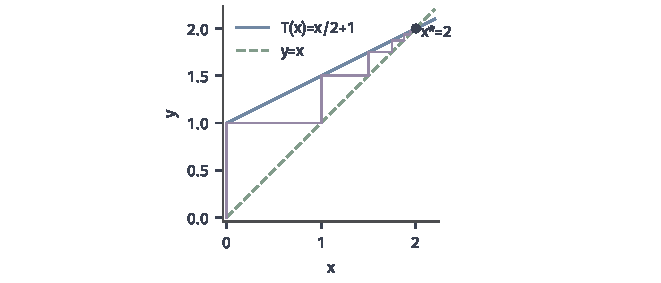
\includegraphics[width=112mm]{figures/01-mathematical-preliminaries-upper/01-mathematical-language-combinatorics-analysis-optimization/matplotlib/comprehension-additions/contraction-cobweb.pdf}
  \caption{$T(x)=x/2+1$在$[0,2]$上的七步迭代，初值$x^{(0)}=0$。蓝线是$T$，绿虚线是恒等函数，紫折线交替完成求值与复制；交点为$x^\star=2$。精确迭代为$x^{(n)}=2-2^{1-n}$，图中几何收缩对应压缩因子$1/2$。}
  \label{fig:vol1-add-contraction-cobweb}
\end{figure}

\paragraph{隐式方程的局部不动点构造}

现在可以补全定理~\ref{thm:analysis-implicit-function}的构造证明。把方程的线性化逆作为校正，使待解变量上的更新在基点处导数为零；再缩小邻域，同时核对统一压缩与自映射。这个顺序同时保证解存在、局部唯一和可微，形式求导只能给出最后的候选公式。

\begin{proof}
为证明定理~\ref{thm:analysis-implicit-function}的存在性，先把方程改写为局部压缩迭代。记
\[   \bm{A}   =   \bm{D}_{\bm{y}}F(\bm{a},\bm{b}),   \qquad   T_{\bm{x}}(\bm{y})   =   \bm{y}-\bm{A}^{-1}F(\bm{x},\bm{y}). \]
$F(\bm{x},\bm{y})=\bm{0}$当且仅当$\bm{y}$是$T_{\bm{x}}$的不动点。并且
\[   \bm{D}_{\bm{y}}T_{\bm{x}}(\bm{y})   =   \bm{I}   -   \bm{A}^{-1}\bm{D}_{\bm{y}}F(\bm{x},\bm{y}), \]
它在$(\bm{a},\bm{b})$处为零。由导数连续性，可以选择闭球 $B=\{\bm{y}:\lVert\bm{y}-\bm{b}\rVert_2\leq r\}$和$\bm{a}$的邻域$U$，使
\begin{equation}
  \sup_{\bm{x}\in U,\,\bm{y}\in B}
  \left\lVert
    \bm{D}_{\bm{y}}T_{\bm{x}}(\bm{y})
  \right\rVert_{\mathrm{op}}
  \leq q<1.
\label{eq:analysis-ift-uniform-contraction}
\end{equation}
沿$\bm{y}$方向使用式~\eqref{eq:analysis-operator-mean-value-bound}可知，每个
$T_{\bm{x}}$在$B$上都是同一因子$q$的压缩映射。

还必须核对自映射。因为$T_{\bm{a}}(\bm{b})=\bm{b}$且$T_{\bm{x}}(\bm{b})$关于 $\bm{x}$连续，可进一步缩小$U$，使
\[   \lVert T_{\bm{x}}(\bm{b})-\bm{b}\rVert_2   \leq\frac{1-q}{2}r. \]
于是对$\bm{y}\in B$，
\[
  \lVert T_{\bm{x}}(\bm{y})-\bm{b}\rVert_2
  \leq
  q\lVert\bm{y}-\bm{b}\rVert_2+\frac{1-q}{2}r
  \leq
  \frac{1+q}{2}r
  <r.
\]
所以$T_{\bm{x}}(B)$包含在$B$的内部$V$中。闭球$B$在有限维欧氏空间中完备，Banach
定理便对每个$\bm{x}\in U$给出唯一不动点$\varphi(\bm{x})\in V$。若
$(\bm{x},\bm{y})\in U\times V$且$F(\bm{x},\bm{y})=\bm{0}$，则$\bm{y}\in B$也是
$T_{\bm{x}}$的不动点，唯一性迫使$\bm{y}=\varphi(\bm{x})$。这证明了定理所述的局部
存在与零点集合的逐点唯一性。

还需说明所得解随参数连续可微。把$U$进一步缩小为开球，并使
$\overline U\times B$包含在原定义域内；这个集合紧致，关于$\bm x$的导数连续，
故有统一范数上界$L$。对$\bm x,\bm x'\in U$，
两点间的线段仍在$U$内，式~\eqref{eq:analysis-operator-mean-value-bound}
可用于$T_{\bm x}(\bm y)$的参数变化。利用两个不动点关系，
\[   \lVert\varphi(\bm{x})-\varphi(\bm{x}')\rVert_2   \leq   q\lVert\varphi(\bm{x})-\varphi(\bm{x}')\rVert_2   +L\lVert\bm{x}-\bm{x}'\rVert_2, \]
移项得到$\lVert\varphi(\bm x)-\varphi(\bm x')\rVert_2
\leq L\lVert\bm x-\bm x'\rVert_2/(1-q)$，
故$\varphi$局部Lipschitz连续。令 $\bm{h}\to\bm{0}$并记 $\bm{k}=\varphi(\bm{x}+\bm{h})-\varphi(\bm{x})$，前述界给出 $\lVert\bm{k}\rVert_2=O(\lVert\bm{h}\rVert_2)$。对恒等式
\[   F(\bm{x}+\bm{h},\varphi(\bm{x})+\bm{k})   -   F(\bm{x},\varphi(\bm{x}))   =   \bm{0} \]
作一阶展开，得到
\[   \bm{D}_{\bm{x}}F\,\bm{h}   +   \bm{D}_{\bm{y}}F\,\bm{k}   +   o(\lVert\bm{h}\rVert_2)   =   \bm{0}. \]
展开中的Jacobian均在$(\bm x,\varphi(\bm x))$处取值，联合扰动的余项
$o(\lVert(\bm h,\bm k)\rVert_2)$因$\lVert\bm k\rVert_2=O(\lVert\bm h\rVert_2)$
成为$o(\lVert\bm h\rVert_2)$。
基点的$\det\bm A\neq0$，行列式又是矩阵元素的连续函数，
所以邻域足够小时$\bm D_{\bm y}F$仍可逆。于是
\[   \bm{k}   =   -   (\bm{D}_{\bm{y}}F)^{-1}   \bm{D}_{\bm{x}}F\,\bm{h}   +   o(\lVert\bm{h}\rVert_2). \]
这证明$\varphi$可微并给出式~\eqref{eq:analysis-implicit-derivative}；各Jacobian矩阵连续又保证$\bm{D}\varphi$连续。至此，隐函数定理中的存在、局部唯一与导数公式都已得到说明。证明中特别核对了自映射和统一压缩条件，只有形式上的固定点改写并不足够。
\end{proof}

\subsubsection{带扰动更新的误差累计}

\paragraph{单步误差的传播权重}

精确更新的压缩性不代表数值实现没有误差。实际迭代几乎总有偏差：用小批量样本估计的更新方向、
浮点舍入、提前停止都会让每一步没有恰好落在$T(x^{(t)})$上。需要回答的是，这些每轮新增的
偏差会被迭代逐步消化，还是累积成一个无法消除的误差底。设$T$满足压缩条件，精确轨迹为
$x^{(t+1)}=T(x^{(t)})$，计算轨迹为$z^{(t)}$，且每次更新满足
$d(z^{(t+1)},T(z^{(t)}))\leq\delta_t$，其中$\delta_t\geq0$。
令$e^{(t)}=d(z^{(t)},x^{(t)})$，三角不等式给出
\begin{equation}
 \begin{aligned}
 e^{(t+1)}
 &\leq d(z^{(t+1)},T(z^{(t)}))
       +d(T(z^{(t)}),T(x^{(t)}))\\
 &\leq\delta_t+\rho e^{(t)},\qquad 0\leq\rho<1.
 \end{aligned}
\label{eq:analysis-perturbed-distance-recursion}
\end{equation}
这里$\rho$就是所用压缩因子。对到不动点的误差$d(z^{(t)},x^\star)$也有同一递推。
把不等式逐次代入，或对$t$归纳，得到
\begin{equation}
 e^{(t)}
 \leq \rho^t e^{(0)}
       +\sum_{s=0}^{t-1}\rho^{t-1-s}\delta_s.
\label{eq:analysis-perturbed-distance-unrolling}
\end{equation}
这正是第~\ref{chap:sets-functions-and-proofs}章式~\eqref{eq:prelim-unrolled-recurrence}
的有限展开在距离误差中的应用；本章再判断它随$t$增加的行为。
若$\delta_s\leq\bar\delta$，则
$e^{(t)}\leq\rho^t e^{(0)}+\bar\delta(1-\rho^t)/(1-\rho)$，
所以$\limsup_t e^{(t)}\leq\bar\delta/(1-\rho)$。
这是最坏误差范围，不是断言每条计算轨迹都收敛到这个上界。

\paragraph{持续扰动与衰减扰动}

展开式中的旧误差会衰减，每轮新增误差则继续进入累计。固定初值与压缩系数，只改变新增误差是否趋零，就能看清两种误差来源。
\begin{example}[持续扰动与衰减扰动]
\label{ex:prelim-recurring-perturbations}
取$e^{(0)}=1$、$\rho=1/2$，并暂把递推中的不等号取为等号。若每步都加入
$\delta_t=0.1$，展开式给出
\[
 e^{(t)}=2^{-t}+0.1\sum_{s=0}^{t-1}2^{-s}
        =0.2+0.8\,2^{-t}.
\]
初始误差逐步消失，持续加入的误差却留下$0.2$的极限。若改为
$\delta_t=0.1/(t+1)$，扰动本身也衰减，稳定递推便使$e^{(t)}\to0$。
例如第$1$步两者都是$0.6$，第$2$步分别为$0.4$和$0.35$；差别来自第二步加入的
新误差，而不是初值不同。这里的$1/(t+1)$扰动并不可求和，几何权重仍能使其累计影响趋于零；可求和性是更强的条件。
\end{example}

\begin{figure}[htbp]
  \centering
  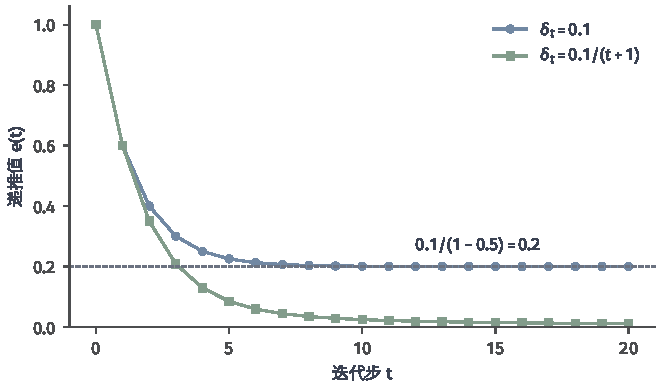
\includegraphics[width=112.0mm]{figures/01-mathematical-preliminaries-upper/01-mathematical-language-combinatorics-analysis-optimization/matplotlib/prelim-perturbed-recurrence/figure.pdf}
  \caption{相同初值与收缩系数下的两种递推。蓝线使用持续扰动，绿线使用衰减扰动；每个点都是整数步上的精确递推值，图中$e(t)$对应正文的$e^{(t)}$，灰虚线是持续扰动留下的极限$0.2$。图为教学构造。}
 \label{fig:prelim-perturbed-recurrence}
\end{figure}

衰减扰动的结论可以直接由有限展开式~\eqref{eq:analysis-perturbed-distance-unrolling}核对。
给定$\varepsilon>0$，先选$S$使$s\geq S$时$\delta_s\leq\varepsilon(1-\rho)/2$。
对$t>S$把累计和拆成两段：前$S$项是有限个旧扰动，其权重随$t$几何趋零；后面的项满足
\[
 \sum_{s=S}^{t-1}\rho^{t-1-s}\delta_s
 \leq\frac{\varepsilon(1-\rho)}2\sum_{j=0}^{t-1-S}\rho^j
 \leq\frac\varepsilon2.
\]
旧扰动项和初始误差在充分大的$t$后也不超过$\varepsilon/2$，因此总误差趋于零。
这里需要$0\leq\rho<1$、$\delta_s\to0$和有限的初始误差；只写“每步误差很小”仍不足够。

函数逼近还可能超出原积分范围。枚举$[0,1]$内的有理数为$q_1,q_2,\ldots$，令$E_n=\{q_1,\ldots,q_n\}$，$g_n=\mathbb I_{E_n}$。每个$g_n$仅在有限个位置不连续，黎曼积分为零；它逐点递增到$d=\mathbb I_{\mathbb Q\cap[0,1]}$，而第~\ref{sec:analysis-riemann-integral}节已证明$d$不黎曼可积。这次困难是极限对象失去原来的可积性；连续尖峰的极限仍然可积，却发生积分交换失败。下一章需要分别扩大积分范围，并建立对整个逼近过程的控制条件。

\section{本章小结}
\label{sec:analysis-summary}

距离说明何谓接近，完备性保证柯西逼近的终点仍在空间内，闭性则保留额外的范围约束。连续性把输入极限传到输出，紧致定义域进一步提供极值达到和统一变化控制。微分在此基础上描述局部变化，有限位移与高阶近似还需要导数界和余项条件。

积分从有限分割的共同累计建立。连续性保证紧区间上的黎曼可积，却不是可积性的必要条件；换元、分部积分及边界公式分别保留体积权重、端点项和法向方向。它们共同把局部变化联系到整体累计，所采用的经典版本均有明确的范围与光滑性条件。

函数列把这些条件重新放到极限中检验。一致误差能保留连续性及有限区间上的积分，却不能独自保证求导交换；导数一致误差还需一个位置的函数值作为锚点。部分和与压缩迭代利用各自生成结构提供误差界，扰动递推则区分单步误差与累计影响。有限点示性函数列和连续尖峰留下两项任务：为更多极限函数建立积分，并控制贡献随逼近移动、集中或消失的情形。这将成为可测函数章的起点。
